\chapter{Diseño de clases} \label{cap:diseño_clases}

\section{Introducción}

En este capítulo se realizará una breve introducción sobre el diagrama de clases y posteriormente, un análisis de las clases que participan en el modelo de información del simulador SimAS 3.0. Para ello, se especificarán los atributos, métodos y las relaciones existentes entre las mismas, terminándose con un diagrama de clases general de todo el sistema.

El propósito de un diagrama de clases es el de representar los objetos fundamentales del sistema, es decir, los que percibe el usuario y con los que espera tratar para completar su tarea. Una clase define el ámbito de definición de un conjunto de objetos.

Cada clase se representa en un rectángulo con tres apartados:
\begin{itemize}
\item Nombre de la clase.
\item Atributos de la clase.
\item Operaciones de la clase.
\end{itemize}

En SimAS 3.0, el diseño de clases sigue el patrón Model-View-Controller (MVC), donde las clases del modelo representan la lógica de negocio y los datos de las gramáticas de contexto libre, mientras que las clases de la vista y controlador manejan la interfaz de usuario y la interacción con el usuario.


\section{Diseño de clases por paquetes}

El sistema SimAS 3.0 está organizado en 8 paquetes principales que contienen un total de 51 clases Java. Para una mejor comprensión y organización, este capítulo presenta las clases agrupadas por paquetes, siguiendo la arquitectura por capas definida en el Capítulo 8.

Cada sección dedicada a un paquete incluye:
\begin{itemize}
    \item \textbf{Introducción}: propósito y responsabilidad del paquete.
    \item \textbf{Clases principales}: análisis detallado de cada clase con atributos y métodos.
    \item \textbf{Dependencias internas}: relaciones entre clases dentro del paquete.
    \item \textbf{Patrones de diseño}: patrones utilizados en el paquete.
\end{itemize}

\subsection{Paquete bienvenida}

El paquete \textbf{bienvenida} contiene las clases responsables de la inicialización y navegación principal de la aplicación SimAS 3.0. Este paquete implementa el patrón Singleton y Facade para gestionar el ciclo de vida de la aplicación.

\subsubsection{Clases del paquete bienvenida}

Este paquete contiene 2 clases principales que gestionan el punto de entrada y la navegación inicial del sistema.

\subsubsection{Clase Bienvenida}

Esta clase representa la pantalla de bienvenida de la aplicación SimAS 3.0, heredando de Application para ser el punto de entrada principal. La implementación actual es simple y delega la interfaz gráfica a un archivo FXML.

\begin{longtable}[H]{|>{\columncolor[rgb]{0.63,0.79,0.95}}m{6cm} | m{8.5cm} |}
 \caption{Clase Bienvenida}

\endfirsthead

\multicolumn{2}{c}
{{\tablename\ \thetable{} -- continúa de la página anterior}} \\
\endhead

\hline \multicolumn{2}{|r|}{{Continúa en la página siguiente}} \\ \hline
\endfoot

\hline
\endlastfoot

\hline
 \textbf{Nombre} & \textbf{Bienvenida}  \\ \hline
 
 \textbf{Descripción} & Representa la pantalla de bienvenida de la aplicación. Es el punto de entrada principal que carga la interfaz desde un archivo FXML y transita al menú principal después de un tiempo determinado.  \\ \hline

 \textbf{Atributos} & La clase no define atributos específicos, ya que la interfaz está definida en el archivo FXML correspondiente. \\ \hline
 
\textbf{Métodos} & \begin{enumerate}
 		\item \textbf{start(Stage)}: método principal que inicializa la aplicación, carga la interfaz FXML y configura la transición automática al menú principal.
 		\item \textbf{main(String[])}: punto de entrada estático de la aplicación JavaFX.
 		\item \textbf{abrirMenuPrincipal()}: método privado que crea y muestra la ventana del menú principal.
\end{enumerate} \\ \hline

 \label{tabla99}

\end{longtable}

\subsubsection{Clase MenuPrincipal}

La clase \textbf{MenuPrincipal} gestiona la interfaz principal de navegación de la aplicación SimAS 3.0, proporcionando acceso a todas las funcionalidades principales del sistema. Implementa un sistema avanzado de pestañas con soporte para arrastrar y soltar, internacionalización completa y gestión de múltiples ventanas.

\begin{longtable}[H]{|>{\columncolor[rgb]{0.63,0.79,0.95}}m{6cm} | m{8.5cm} |}
\caption{Clase MenuPrincipal - Interfaz principal de navegación}
\endfirsthead
\multicolumn{2}{c}{{\tablename\ \thetable{} -- continúa de la página anterior}} \\
\endhead
\hline \multicolumn{2}{|r|}{{Continúa en la página siguiente}} \\ \hline
\endfoot
\hline
\endlastfoot
\hline
\textbf{Nombre} & \textbf{MenuPrincipal} \\ \hline
\textbf{Descripción} & Gestiona el menú principal de navegación con sistema de pestañas avanzado, internacionalización y gestión de módulos. \\ \hline
\textbf{Atributos} &
\begin{enumerate}
    \item \textbf{tabPane}: TabPane que contiene todas las pestañas de edición y simulación.
    \item \textbf{mainTab}: pestaña principal del menú.
    \item \textbf{btnCerrarTabs}: botón para cerrar todas las pestañas.
    \item \textbf{comboIdioma}: ComboBox para selección de idioma.
    \item \textbf{btnEditor}: botón para abrir el editor de gramáticas.
    \item \textbf{btnSalir}: botón para salir de la aplicación.
    \item \textbf{btnSimulador}: botón para abrir el simulador.
    \item \textbf{btnAyuda}: botón para abrir la ayuda.
    \item \textbf{btnTutorial}: botón para abrir el tutorial.
    \item \textbf{labelTitulo}: etiqueta con el título de la aplicación.
    \item \textbf{labelSubtitulo}: etiqueta con el subtítulo.
    \item \textbf{labelDesarrollado}: etiqueta con información del desarrollador.
    \item \textbf{lastSelectedTab}: referencia a la última pestaña seleccionada.
    \item \textbf{bundle}: ResourceBundle para internacionalización.
    \item \textbf{currentLocale}: Locale actual de la aplicación.
\end{enumerate} \\ \hline
\textbf{Métodos} &
\begin{enumerate}
    \item \textbf{start(Stage)}: método principal que inicializa la interfaz del menú con configuración completa.
    \item \textbf{main(String[])}: punto de entrada alternativo de la aplicación.
    \item \textbf{initialize()}: método de inicialización FXML que configura componentes y eventos.
    \item \textbf{cambiarIdioma()}: cambia el idioma de la aplicación basado en la selección del usuario.
    \item \textbf{cargarBundle(Locale)}: carga el ResourceBundle para el idioma especificado.
    \item \textbf{actualizarTextos()}: actualiza todos los textos de la interfaz según el bundle actual.
    \item \textbf{sincronizarIdiomaConVentanas Secundarias()}: sincroniza el cambio de idioma con todas las ventanas secundarias activas.
    \item \textbf{actualizarTodosLosSimuladores()}: actualiza el bundle de todos los simuladores activos.
    \item \textbf{onBtnCerrarTabsAction()}: maneja el cierre de todas las pestañas con confirmación.
    \item \textbf{onBtnEditorAction()}: abre una nueva instancia del editor de gramáticas.
    \item \textbf{onBtnAyudaAction()}: abre el manual de usuario en el navegador.
    \item \textbf{onBtnTutorialAction()}: abre el tutorial interactivo.
    \item \textbf{onBtnSimuladorAction()}: carga una gramática y abre el simulador directamente.
\end{enumerate} \\ \hline
\textbf{Métodos} &
\begin{enumerate}
    \item \textbf{cargarGramaticaYSimular Directamente()}: proceso completo para cargar gramática y crear simulador.
    \item \textbf{crearSimuladorDirectoAlPaso6( Gramatica)}: crea simulador y lo posiciona en el paso 6.
    \item \textbf{mostrarErroresValidacion( ObservableList<String>)}: muestra errores de validación en diálogo.
    \item \textbf{mostrarError(String, String)}: muestra mensaje de error genérico.
    \item \textbf{onMostrarErrorAction(String)}: muestra alerta de error para operaciones fallidas.
    \item \textbf{onBtnSalirAction()}: maneja la salida de la aplicación con confirmación.
    \item \textbf{onBtnInfoAction()}: muestra información "Acerca de" de la aplicación.
    \item \textbf{setBundle(ResourceBundle)}: establece un nuevo bundle y actualiza textos.
    \item \textbf{actualizarTextos(ResourceBundle)}: sobrecarga para actualizar textos con bundle específico.
    \item \textbf{reasignarNumerosSimulaciones( TabPane)}: reasigna números de simulación tras cambios.
    \item \textbf{findFirstTabInGroup(TabPane, int)}: encuentra la primera pestaña de un grupo específico.
\end{enumerate} \\ \hline
\label{tabla_menu_principal}
\end{longtable}

\subsubsection{Dependencias internas del paquete bienvenida}

\begin{itemize}
    \item \textbf{Bienvenida $\rightarrow$ MenuPrincipal}: la clase Bienvenida crea y transita hacia MenuPrincipal después de mostrar la pantalla de bienvenida.
    \item \textbf{MenuPrincipal $\rightarrow$ Editor}: MenuPrincipal crea instancias del Editor para edición de gramáticas.
    \item \textbf{MenuPrincipal $\rightarrow$ PanelSimuladorDesc}: MenuPrincipal crea instancias del simulador descendente.
    \item \textbf{MenuPrincipal $\rightarrow$ SecondaryWindow}: MenuPrincipal puede crear ventanas secundarias para gestión de pestañas.
    \item \textbf{MenuPrincipal $\rightarrow$ TabManager}: MenuPrincipal utiliza TabManager para gestión avanzada de pestañas.
    \item \textbf{MenuPrincipal $\rightarrow$ LanguageItem}: MenuPrincipal utiliza LanguageItem para el selector de idiomas.
    \item \textbf{MenuPrincipal $\rightarrow$ ResourceBundle}: MenuPrincipal gestiona la internacionalización mediante ResourceBundle.
\end{itemize}

\subsubsection{Patrones de diseño en el paquete bienvenida}

\begin{itemize}
    \item \textbf{Facade}: MenuPrincipal actúa como fachada simplificando el acceso a los módulos complejos del sistema (editor, simulador, ayuda) \cite{gamma1995design}.
    \item \textbf{Observer}: MenuPrincipal implementa el patrón Observer para actualizar textos cuando cambia el idioma \cite{gamma1995design}.
    \item \textbf{Factory Method}: Los métodos de creación de editores y simuladores siguen el patrón Factory Method \cite{gamma1995design}.
    \item \textbf{Strategy}: La gestión de diferentes tipos de módulos (editores, simuladores) utiliza el patrón Strategy \cite{gamma1995design}.
\end{itemize}

\subsection{Paquete gramática}

El paquete \textbf{gramática} contiene las clases fundamentales que representan el modelo de datos del simulador SimAS 3.0. Este paquete implementa el patrón de diseño Modelo-Vista-Controlador (MVC) donde las clases del modelo encapsulan toda la lógica de negocio relacionada con las gramáticas de contexto libre, incluyendo su definición, manipulación y análisis sintáctico.

Las clases de este paquete permiten:
\begin{itemize}
    \item Definir y manipular símbolos terminales y no terminales
    \item Crear y gestionar producciones gramaticales
    \item Construir y consultar tablas predictivas para análisis sintáctico
    \item Gestionar funciones de error para recuperación de errores
    \item Integración completa con la interfaz JavaFX mediante propiedades observables
\end{itemize}

\subsubsection{Clases del paquete gramática}

Este paquete contiene 11 clases principales que conforman el núcleo del modelo de datos de SimAS 3.0, organizadas jerárquicamente desde los elementos básicos hasta las estructuras complejas de análisis. Las clases se presentan en orden lógico de dependencia, desde las más básicas hasta las más complejas.

\subsubsection{Clase Simbolo}

La clase \textbf{Simbolo} es la clase base abstracta que representa cualquier símbolo en una gramática de contexto libre, sirviendo como superclase para Terminal y NoTerminal.

\begin{longtable}[H]{|>{\columncolor[rgb]{0.63,0.79,0.95}}m{6cm} | m{8.5cm} |}
\caption{Clase Simbolo - Clase base para símbolos gramaticales}
\endfirsthead
\multicolumn{2}{c}{{\tablename\ \thetable{} -- continúa de la página anterior}} \\
\endhead
\hline \multicolumn{2}{|r|}{{Continúa en la página siguiente}} \\ \hline
\endfoot
\hline
\endlastfoot
\hline
\textbf{Nombre} & \textbf{Simbolo} \\ \hline
\textbf{Descripción} & Clase base abstracta que representa un símbolo genérico en la gramática, proporcionando la estructura común para terminales y no terminales. \\ \hline
\textbf{Atributos} &
\begin{enumerate}
    \item \textbf{nombre}: StringProperty que contiene el nombre/valor del símbolo.
    \item \textbf{valor}: StringProperty que contiene información adicional del símbolo.
\end{enumerate} \\ \hline
\textbf{Métodos} &
\begin{enumerate}
    \item \textbf{Simbolo(String, String)}: constructor que inicializa nombre y valor.
    \item \textbf{getNombre()}: obtiene el nombre del símbolo.
    \item \textbf{setNombre(String)}: establece el nombre del símbolo.
    \item \textbf{nombreProperty()}: devuelve la propiedad observable del nombre.
    \item \textbf{getValor()}: obtiene el valor del símbolo.
    \item \textbf{setValor(String)}: establece el valor del símbolo.
    \item \textbf{valorProperty()}: devuelve la propiedad observable del valor.
\end{enumerate}
\label{tabla_simbolo}
\end{longtable}

\subsubsection{Clase Terminal}

La clase \textbf{Terminal} representa un símbolo terminal en la gramática, heredando de la clase Simbolo.

\begin{longtable}[H]{|>{\columncolor[rgb]{0.63,0.79,0.95}}m{6cm} | m{8.5cm} |}
\caption{Clase Terminal - Símbolos terminales de la gramática}
\endfirsthead
\multicolumn{2}{c}{{\tablename\ \thetable{} -- continúa de la página anterior}} \\
\endhead
\hline \multicolumn{2}{|r|}{{Continúa en la página siguiente}} \\ \hline
\endfoot
\hline
\endlastfoot
\hline
\textbf{Nombre} & \textbf{Terminal} \\ \hline
\textbf{Descripción} & Representa un símbolo terminal de la gramática, que son los símbolos básicos que no pueden ser reemplazados por otros símbolos. \\ \hline
\textbf{Atributos} & Hereda todos los atributos de Simbolo (nombre, valor). \\ \hline
\textbf{Métodos} &
\begin{enumerate}
    \item \textbf{Terminal(String, String)}: constructor que inicializa el terminal con nombre y valor.
    \item \textbf{toString()}: devuelve el nombre del terminal para representación textual.
\end{enumerate}
\label{tabla_terminal}
\end{longtable}

\subsubsection{Clase NoTerminal}

La clase \textbf{NoTerminal} representa un símbolo no terminal en la gramática, heredando de Simbolo y añadiendo funcionalidades específicas para el análisis sintáctico.

\begin{longtable}[H]{|>{\columncolor[rgb]{0.63,0.79,0.95}}m{6cm} | m{8.5cm} |}
\caption{Clase NoTerminal - Símbolos no terminales de la gramática}
\endfirsthead
\multicolumn{2}{c}{{\tablename\ \thetable{} -- continúa de la página anterior}} \\
\endhead
\hline \multicolumn{2}{|r|}{{Continúa en la página siguiente}} \\ \hline
\endfoot
\hline
\endlastfoot
\hline
\textbf{Nombre} & \textbf{NoTerminal} \\ \hline
\textbf{Descripción} & Representa un símbolo no terminal de la gramática, que puede ser reemplazado por secuencias de otros símbolos durante el análisis sintáctico. \\ \hline
\textbf{Atributos} &
\begin{enumerate}
    \item \textbf{simboloInicial}: boolean que indica si este no terminal es el símbolo inicial de la gramática.
    \item \textbf{primeros}: ObservableList de Terminal que contiene el conjunto primeros del no terminal.
    \item \textbf{siguientes}: ObservableList de Terminal que contiene el conjunto siguientes del no terminal.
\end{enumerate} \\ \hline
\textbf{Métodos} &
\begin{enumerate}
    \item \textbf{NoTerminal(String, String)}: constructor que inicializa el no terminal.
    \item \textbf{setSimboloInicial(boolean)}: marca este no terminal como símbolo inicial.
    \item \textbf{getSimboloInicial()}: verifica si es el símbolo inicial.
    \item \textbf{getPrimeros()}: obtiene el conjunto primeros.
    \item \textbf{setPrimeros( ObservableList<Terminal>)}: establece el conjunto primeros.
    \item \textbf{getSiguientes()}: obtiene el conjunto siguientes.
    \item \textbf{setSiguientes( ObservableList<Terminal>)}: establece el conjunto siguientes.
    \item \textbf{toString()}: devuelve el nombre del no terminal.
\end{enumerate}
\label{tabla_no_terminal}
\end{longtable}

\subsubsection{Clase Consecuente}

La clase \textbf{Consecuente} representa la parte derecha de una producción gramatical, conteniendo la secuencia de símbolos que reemplaza al antecedente.

\begin{longtable}[H]{|>{\columncolor[rgb]{0.63,0.79,0.95}}m{6cm} | m{8.5cm} |}
\caption{Clase Consecuente - Parte derecha de las producciones}
\endfirsthead
\multicolumn{2}{c}{{\tablename\ \thetable{} -- continúa de la página anterior}} \\
\endhead
\hline \multicolumn{2}{|r|}{{Continúa en la página siguiente}} \\ \hline
\endfoot
\hline
\endlastfoot
\hline
\textbf{Nombre} & \textbf{Consecuente} \\ \hline
\textbf{Descripción} & Representa el consecuente (lado derecho) de una producción gramatical, compuesto por una secuencia ordenada de símbolos. \\ \hline
\textbf{Atributos} &
\begin{enumerate}
    \item \textbf{conjSimbolos}: ObservableList de Simbolo que contiene la secuencia de símbolos del consecuente.
\end{enumerate} \\ \hline
\textbf{Métodos} &
\begin{enumerate}
    \item \textbf{Consecuente()}: constructor sin parámetros que inicializa la lista vacía.
    \item \textbf{getConjSimbolos()}: obtiene la lista de símbolos del consecuente.
    \item \textbf{setConjSimbolos(ObservableList <Simbolo>)}: establece la lista de símbolos del consecuente.
\end{enumerate}
\label{tabla_consecuente}
\end{longtable}

\subsubsection{Clase Antecedente}

La clase \textbf{Antecedente} representa la parte izquierda de una producción gramatical, conteniendo el símbolo no terminal que será reemplazado.

\begin{longtable}[H]{|>{\columncolor[rgb]{0.63,0.79,0.95}}m{6cm} | m{8.5cm} |}
\caption{Clase Antecedente - Parte izquierda de las producciones}
\endfirsthead
\multicolumn{2}{c}{{\tablename\ \thetable{} -- continúa de la página anterior}} \\
\endhead
\hline \multicolumn{2}{|r|}{{Continúa en la página siguiente}} \\ \hline
\endfoot
\hline
\endlastfoot
\hline
\textbf{Nombre} & \textbf{Antecedente} \\ \hline
\textbf{Descripción} & Representa el antecedente (lado izquierdo) de una producción gramatical, compuesto por un único símbolo no terminal. \\ \hline
\textbf{Atributos} &
\begin{enumerate}
    \item \textbf{simboloNT}: NoTerminal que representa el símbolo no terminal del antecedente.
\end{enumerate} \\ \hline
\textbf{Métodos} &
\begin{enumerate}
    \item \textbf{Antecedente()}: constructor sin parámetros que inicializa con valores vacíos.
    \item \textbf{Antecedente(NoTerminal)}: constructor con símbolo no terminal específico.
    \item \textbf{getSimboloNT()}: obtiene el símbolo no terminal del antecedente.
    \item \textbf{setSimboloNT(NoTerminal)}: establece el símbolo no terminal del antecedente.
    \item \textbf{toString()}: devuelve la representación textual del antecedente.
\end{enumerate}
\label{tabla_antecedente}
\end{longtable}

\subsubsection{Clase Produccion}

La clase \textbf{Produccion} representa una regla completa de producción en la gramática, compuesta por un antecedente y un consecuente.

\begin{longtable}[H]{|>{\columncolor[rgb]{0.63,0.79,0.95}}m{6cm} | m{8.5cm} |}
\caption{Clase Produccion - Reglas de producción gramatical}
\endfirsthead
\multicolumn{2}{c}{{\tablename\ \thetable{} -- continúa de la página anterior}} \\
\endhead
\hline \multicolumn{2}{|r|}{{Continúa en la página siguiente}} \\ \hline
\endfoot
\hline
\endlastfoot
\hline
\textbf{Nombre} & \textbf{Produccion} \\ \hline
\textbf{Descripción} & Representa una producción completa de la gramática, formada por un antecedente y un consecuente (secuencia de símbolos). \\ \hline
\textbf{Atributos} &
\begin{enumerate}
    \item \textbf{antec}: Antecedente que contiene el símbolo no terminal de la izquierda.
    \item \textbf{consec}: ObservableList de Simbolo que contiene la secuencia de símbolos del lado derecho.
    \item \textbf{numero}: int que identifica el número de la producción en la gramática.
\end{enumerate} \\ \hline
\textbf{Métodos} &
\begin{enumerate}
    \item \textbf{Produccion()}: constructor sin parámetros con inicialización básica.
    \item \textbf{Produccion(Antecedente, ObservableList<Simbolo>)}: constructor completo.
    \item \textbf{getAntec()}: obtiene el antecedente de la producción.
    \item \textbf{setAntec(Antecedente)}: establece el antecedente.
    \item \textbf{getConsec()}: obtiene el consecuente (lista de símbolos).
    \item \textbf{setConsec( ObservableList<Simbolo>)}: establece el consecuente.
    \item \textbf{getNumero()}: obtiene el número de la producción.
    \item \textbf{setNumero(int)}: establece el número de la producción.
    \item \textbf{toString()}: devuelve la representación textual completa de la producción.
    \item \textbf{modificarSimbolo(String, String)}: modifica símbolos en la producción.
\end{enumerate}
\label{tabla_produccion}
\end{longtable}

\subsubsection{Clase Gramatica}

La clase \textbf{Gramatica} representa el núcleo del modelo de datos de SimAS 3.0, encapsulando toda la información y funcionalidad relacionada con una gramática de contexto libre.

\begin{longtable}[H]{|>{\columncolor[rgb]{0.63,0.79,0.95}}m{6cm} | m{8.5cm} |}
\caption{Clase Gramatica - Núcleo del modelo de datos}
\endfirsthead
\multicolumn{2}{c}{{\tablename\ \thetable{} -- continúa de la página anterior}} \\
\endhead
\hline \multicolumn{2}{|r|}{{Continúa en la página siguiente}} \\ \hline
\endfoot
\hline
\endlastfoot
\hline
\textbf{Nombre} & \textbf{Gramatica} \\ \hline
\textbf{Descripción} & Clase central que representa una gramática de contexto libre completa con todas sus propiedades y métodos de manipulación. \\ \hline
\textbf{Atributos} &
\begin{enumerate}
    \item \textbf{nombre}: StringProperty para el nombre de la gramática.
    \item \textbf{descripcion}: StringProperty para la descripción de la gramática.
    \item \textbf{simbInicial}: StringProperty para el símbolo inicial.
    \item \textbf{archivoFuente}: StringProperty para el nombre del archivo fuente.
    \item \textbf{estado}: IntegerProperty para el estado actual de la gramática.
    \item \textbf{terminales}: ObservableList de objetos Terminal.
    \item \textbf{noTerminales}: ObservableList de objetos NoTerminal.
    \item \textbf{pr}: ObservableList de objetos Produccion.
    \item \textbf{noTerm}: ObservableList de strings para nombres de no terminales (modelo UI).
    \item \textbf{term}: ObservableList de strings para nombres de terminales (modelo UI).
    \item \textbf{producciones}: ObservableList de strings para representaciones de producciones (modelo UI).
    \item \textbf{tpredictiva}: TablaPredictiva para el análisis sintáctico.
\end{enumerate} \\ \hline
\textbf{Métodos} &
\begin{enumerate}
    \item \textbf{Gramatica()}: constructor sin parámetros con valores por defecto.
    \item \textbf{Gramatica(String, String)}: constructor con nombre y descripción.
    \item \textbf{Gramatica(Gramatica)}: constructor de copia.
    \item \textbf{getNombre()/setNombre()}: getters/setters para el nombre.
    \item \textbf{getDescripcion()/setDescripcion()}: getters/setters para la descripción.
    \item \textbf{getSimbInicial()/setSimbInicial()}: getters/setters para el símbolo inicial.
    \item \textbf{getEstado()/setEstado()}: getters/setters para el estado.
    \item \textbf{getTerminales()}: obtiene la lista de terminales.
    \item \textbf{getNoTerminales()}: obtiene la lista de no terminales.
    \item \textbf{getProducciones()}: obtiene la lista de producciones.
\end{enumerate} \\ \hline
\textbf{Métodos} &
\begin{enumerate}
    \item \textbf{validarGramatica()}: valida que la gramática esté bien formada y retorna lista de errores.
    \item \textbf{guardarGramatica(Window)}: guarda la gramática en un archivo mediante diálogo de selección.
    \item \textbf{cargarGramatica(Window)}: carga una gramática desde archivo mediante diálogo de selección.
    \item \textbf{generarInforme(String)}: genera un informe PDF básico de la gramática.
    \item \textbf{generarInforme(String, ResourceBundle)}: genera un informe PDF con internacionalización.
    \item \textbf{generarNombreArchivoPDF(String, ResourceBundle)}: genera nombre apropiado para archivo PDF según tipo.
    \item \textbf{actualizarNoTerminalesDesdeModel()}: actualiza la lista de no terminales desde el modelo UI.
    \item \textbf{numerarProducciones()}: asigna números secuenciales a todas las producciones.
    \item \textbf{getNumeroProduccion(String)}: obtiene el número de una producción específica.
    \item \textbf{selecSimboloInicial(String)}: selecciona y valida el símbolo inicial.
    \item \textbf{setVocabulario(ObservableList, ObservableList)}: establece el vocabulario de terminales y no terminales.
\end{enumerate}
\label{tabla_gramatica}
\end{longtable}

\subsubsection{Clase FilaTablaPredictiva}

La clase \textbf{FilaTablaPredictiva} representa una fila individual de la tabla predictiva, asociando un símbolo (terminal o no terminal) con sus correspondientes acciones de análisis.

\begin{longtable}[H]{|>{\columncolor[rgb]{0.63,0.79,0.95}}m{6cm} | m{8.5cm} |}
\caption{Clase FilaTablaPredictiva - Filas de la tabla predictiva}
\endfirsthead
\multicolumn{2}{c}{{\tablename\ \thetable{} -- continúa de la página anterior}} \\
\endhead
\hline \multicolumn{2}{|r|}{{Continúa en la página siguiente}} \\ \hline
\endfoot
\hline
\endlastfoot
\hline
\textbf{Nombre} & \textbf{FilaTablaPredictiva} \\ \hline
\textbf{Descripción} & Representa una fila de la tabla predictiva, conteniendo el símbolo no terminal y las acciones correspondientes para cada terminal. \\ \hline
\textbf{Atributos} &
\begin{enumerate}
    \item \textbf{simbolo}: StringProperty que contiene el nombre del símbolo (no terminal).
    \item \textbf{prediccion}: StringProperty que contiene información de predicción.
    \item \textbf{valoresColumnas}: Map dinámico que asocia cada terminal con su acción correspondiente.
    \item \textbf{esTerminal}: BooleanProperty que indica si la fila corresponde a un terminal.
    \item \textbf{celdasConProduccion}: Map que marca qué celdas contienen producciones.
\end{enumerate} \\ \hline
\textbf{Métodos} &
\begin{enumerate}
    \item \textbf{FilaTablaPredictiva(String, String, boolean)}: constructor principal.
    \item \textbf{FilaTablaPredictiva(String, String)}: constructor simplificado.
    \item \textbf{setValor(String, String)}: establece el valor para una columna específica.
    \item \textbf{getValor(String)}: obtiene el valor de una columna específica.
    \item \textbf{setProduccionEnCelda(String, boolean)}: marca si una celda contiene producción.
    \item \textbf{tieneProduccionEnCelda(String)}: verifica si una celda contiene producción.
    \item \textbf{simboloProperty()}: devuelve la propiedad observable del símbolo.
    \item \textbf{esTerminalProperty()}: devuelve la propiedad observable del tipo.
\end{enumerate}
\label{tabla_fila_tabla_predictiva}
\end{longtable}

\subsubsection{Clase FuncionError}

La clase \textbf{FuncionError} representa las funciones de manejo de errores utilizadas durante el análisis sintáctico para recuperación de errores.

\begin{longtable}[H]{|>{\columncolor[rgb]{0.63,0.79,0.95}}m{6cm} | m{8.5cm} |}
\caption{Clase FuncionError - Funciones de manejo de errores}
\endfirsthead
\multicolumn{2}{c}{{\tablename\ \thetable{} -- continúa de la página anterior}} \\
\endhead
\hline \multicolumn{2}{|r|}{{Continúa en la página siguiente}} \\ \hline
\endfoot
\hline
\endlastfoot
\hline
\textbf{Nombre} & \textbf{FuncionError} \\ \hline
\textbf{Descripción} & Representa una función de manejo de errores para recuperación durante el análisis sintáctico predictivo. \\ \hline
\textbf{Atributos} &
\begin{enumerate}
    \item \textbf{identificador}: int que identifica de forma única la función de error.
    \item \textbf{accion}: int que representa el tipo de acción a realizar.
    \item \textbf{mensaje}: String que contiene el mensaje descriptivo del error.
    \item \textbf{simbolo}: Terminal asociado a la función de error.
\end{enumerate} \\ \hline
\textbf{Métodos} &
\begin{enumerate}
    \item \textbf{FuncionError(int, int, String)}: constructor con parámetros.
    \item \textbf{FuncionError()}: constructor sin parámetros.
    \item \textbf{getIdentificador()}: obtiene el identificador único.
    \item \textbf{setIdentificador(int)}: establece el identificador.
    \item \textbf{getAccion()}: obtiene el tipo de acción.
    \item \textbf{setAccion(int)}: establece el tipo de acción.
    \item \textbf{getMensaje()}: obtiene el mensaje de error.
    \item \textbf{setMensaje(String)}: establece el mensaje de error.
    \item \textbf{getSimbolo()}: obtiene el símbolo terminal asociado.
    \item \textbf{setSimbolo(Terminal)}: establece el símbolo terminal.
    \item \textbf{getNombreAccion()}: devuelve el nombre descriptivo de la acción.
    \item \textbf{toString()}: representación textual completa de la función.
\end{enumerate} \\ \hline
\textbf{Constantes de Acción} &
\begin{enumerate}
    \item \textbf{INSERTAR\_ENTRADA}: insertar entrada en el flujo de entrada.
    \item \textbf{BORRAR\_ENTRADA}: borrar entrada del flujo de entrada.
    \item \textbf{MODIFICAR\_ENTRADA}: modificar entrada del flujo de entrada.
    \item \textbf{INSERTAR\_PILA}: insertar elemento en la pila de análisis.
    \item \textbf{BORRAR\_PILA}: borrar elemento de la pila de análisis.
    \item \textbf{MODIFICAR\_PILA}: modificar elemento de la pila de análisis.
    \item \textbf{TERMINAR\_ANALISIS}: terminar el análisis sintáctico.
\end{enumerate}
\label{tabla_funcion_error}
\end{longtable}

\subsubsection{Clase TablaPredictiva}

La clase \textbf{TablaPredictiva} representa la tabla predictiva completa utilizada en el análisis sintáctico LL(1), conteniendo todas las acciones de análisis para cada combinación de no terminal y terminal.

\begin{longtable}[H]{|>{\columncolor[rgb]{0.63,0.79,0.95}}m{6cm} | m{8.5cm} |}
\caption{Clase TablaPredictiva - Tabla de análisis sintáctico}
\endfirsthead
\multicolumn{2}{c}{{\tablename\ \thetable{} -- continúa de la página anterior}} \\
\endhead
\hline \multicolumn{2}{|r|}{{Continúa en la página siguiente}} \\ \hline
\endfoot
\hline
\endlastfoot
\hline
\textbf{Nombre} & \textbf{TablaPredictiva} \\ \hline
\textbf{Descripción} & Representa la tabla predictiva completa para análisis sintáctico LL(1), organizando las acciones de análisis en una estructura tabular. \\ \hline
\textbf{Atributos} &
\begin{enumerate}
    \item \textbf{tablaPredictiva}: TableView que contiene la representación visual de la tabla.
    \item \textbf{gramatica}: referencia a la gramática asociada.
    \item \textbf{indiceColumnas}: Map que asocia nombres de terminales con índices de columna.
    \item \textbf{funcionesError}: List de FuncionError para manejo de errores.
    \item \textbf{bundle}: ResourceBundle para internacionalización.
\end{enumerate} \\ \hline
\textbf{Métodos} &
\begin{enumerate}
    \item \textbf{TablaPredictiva()}: constructor sin parámetros con inicialización básica.
    \item \textbf{TablaPredictiva(TableView)}: constructor con vista de tabla específica.
    \item \textbf{TablaPredictiva(TableView, ResourceBundle)}: constructor completo con internacionalización.
    \item \textbf{construir(Gramatica)}: construye la tabla predictiva completa a partir de una gramática.
    \item \textbf{cargarDatos()}: carga los datos de las filas en la tabla visual (método protegido).
    \item \textbf{crearFunError(FuncionError)}: crea y añade una función de error a la lista.
    \item \textbf{getFuncionesError()}: obtiene la lista de funciones de error.
    \item \textbf{setFuncionesError( List<FuncionError>)}: establece la lista de funciones de error.
    \item \textbf{getTablaPredictiva()}: obtiene la vista de tabla TableView.
    \item \textbf{getFilas()}: obtiene la lista de filas de la tabla.
    \item \textbf{getColumnas()}: obtiene el número de columnas de la tabla.
    \item \textbf{setItems(ObservableList)}: establece los items en la tabla (método protegido).
\end{enumerate}
\label{tabla_tabla_predictiva}
\end{longtable}

\subsubsection{Clase TablaPredictivaPaso5}

La clase \textbf{TablaPredictivaPaso5} es una extensión especializada de TablaPredictiva específica para el paso 5 del simulador, que incluye funcionalidades adicionales para manejo de funciones de error y configuración avanzada de la interfaz.

\begin{longtable}[H]{|>{\columncolor[rgb]{0.63,0.79,0.95}}m{6cm} | m{8.5cm} |}
\caption{Clase TablaPredictivaPaso5 - Tabla predictiva extendida}
\endfirsthead
\multicolumn{2}{c}{{\tablename\ \thetable{} -- continúa de la página anterior}} \\
\endhead
\hline \multicolumn{2}{|r|}{{Continúa en la página siguiente}} \\ \hline
\endfoot
\hline
\endlastfoot
\hline
\textbf{Nombre} & \textbf{TablaPredictivaPaso5} \\ \hline
\textbf{Descripción} & Extensión especializada de TablaPredictiva para el paso 5, incluyendo manejo avanzado de errores y configuración de interfaz específica. \\ \hline
\textbf{Atributos} &
\begin{enumerate}
    \item \textbf{panelPaso5}: referencia al panel específico del paso 5.
    \item \textbf{funcionesError}: List de FuncionError para recuperación de errores.
    \item \textbf{columnsCreated}: boolean que indica si las columnas ya fueron creadas.
\end{enumerate} \\ \hline
\textbf{Métodos} &
\begin{enumerate}
    \item \textbf{TablaPredictivaPaso5()}: constructor sin parámetros con inicialización básica.
    \item \textbf{TablaPredictivaPaso5(TableView)}: constructor con vista de tabla específica.
    \item \textbf{setPanelPaso5( PanelNuevaSimDescPaso5)}: establece el panel del paso 5 asociado.
    \item \textbf{apareceSoloPrimeraPos(Terminal)}: verifica si un terminal aparece solo en primera posición de las producciones.
    \item \textbf{rellenarProduccionesEpsilon()}: rellena automáticamente producciones épsilon en las celdas vacías.
    \item \textbf{construir(Gramatica)}: construye la tabla con lógica específica del paso 5 (override).
    \item \textbf{crearColumnas(Gramatica)}: crea las columnas de la tabla de forma dinámica.
    \item \textbf{cargarDatos()}: carga datos con filas para terminales y no terminales (override).
    \item \textbf{configurarColumnas()}: configura el estilo y comportamiento de las columnas.
    \item \textbf{configurarSeleccion()}: configura la selección de celdas.
    \item \textbf{configurarManejadorClics()}: configura el manejo de eventos de clic en celdas.
    \item \textbf{mostrarError(String, String, String)}: muestra mensajes de error al usuario.
    \item \textbf{setTablaPredictiva(TableView)}: establece la vista de tabla con validaciones.
    \item \textbf{getGramatica()}: obtiene la gramática asociada a esta tabla.
\end{enumerate} \\ \hline
\textbf{Métodos Heredados} &
\begin{enumerate}
    \item \textbf{getFuncionesError()}: obtiene la lista de funciones de error (override).
    \item \textbf{setFuncionesError( List<FuncionError>)}: establece las funciones de error (override).
    \item \textbf{getTablaPredictiva()}: obtiene la vista de tabla TableView.
    \item \textbf{construir(Gramatica)}: construye la tabla predictiva base.
    \item \textbf{cargarDatos()}: carga los datos básicos (método base).
\end{enumerate}
\label{tabla_tabla_predictiva_paso5}
\end{longtable}

\subsubsection{Dependencias internas del paquete gramática}

Las dependencias internas del paquete gramática se muestran en la Figura \ref{fig:diagrama_gramatica}, donde se puede observar la estructura jerárquica y las relaciones entre las diferentes clases.

\begin{itemize}
    \item \textbf{Gramatica $\rightarrow$ Simbolo}: La clase Gramatica contiene listas de Terminal y NoTerminal (que heredan de Simbolo).
    \item \textbf{Gramatica $\rightarrow$ Produccion}: Gramatica mantiene una lista de producciones que definen las reglas gramaticales.
    \item \textbf{Gramatica $\rightarrow$ TablaPredictiva}: Gramatica utiliza TablaPredictiva para el análisis sintáctico.
    \item \textbf{Gramatica $\rightarrow$ FilaTablaPredictiva}: Gramatica crea instancias de FilaTablaPredictiva para la tabla predictiva.
    \item \textbf{Simbolo $\rightarrow$ Terminal, NoTerminal}: Simbolo es la clase base para Terminal y NoTerminal.
    \item \textbf{Produccion $\rightarrow$ Antecedente, Consecuente}: Produccion combina Antecedente y Consecuente.
    \item \textbf{Antecedente $\rightarrow$ NoTerminal}: Antecedente referencia un NoTerminal como símbolo de la izquierda.
    \item \textbf{Consecuente $\rightarrow$ Simbolo}: Consecuente contiene una lista de símbolos (Terminal y NoTerminal).
    \item \textbf{NoTerminal $\rightarrow$ Terminal}: NoTerminal contiene listas de Terminal para conjuntos primeros y siguientes.
    \item \textbf{TablaPredictiva $\rightarrow$ FilaTablaPredictiva}: TablaPredictiva contiene filas de FilaTablaPredictiva.
    \item \textbf{TablaPredictiva $\rightarrow$ FuncionError}: TablaPredictiva gestiona una lista de FuncionError para recuperación de errores.
    \item \textbf{TablaPredictivaPaso5 $\rightarrow$ TablaPredictiva}: TablaPredictivaPaso5 extiende TablaPredictiva con funcionalidades específicas para el paso 5.
    \item \textbf{TablaPredictivaPaso5 $\rightarrow$ PanelNuevaSimDescPaso5}: TablaPredictivaPaso5 interactúa con el panel del paso 5 del simulador.
    \item \textbf{FuncionError $\rightarrow$ Terminal}: FuncionError puede estar asociado con un Terminal específico.
    \item \textbf{FilaTablaPredictiva $\rightarrow$ Terminal}: FilaTablaPredictiva referencia terminales para las columnas de la tabla.
\end{itemize}

\begin{figure}[H]
    \centering
    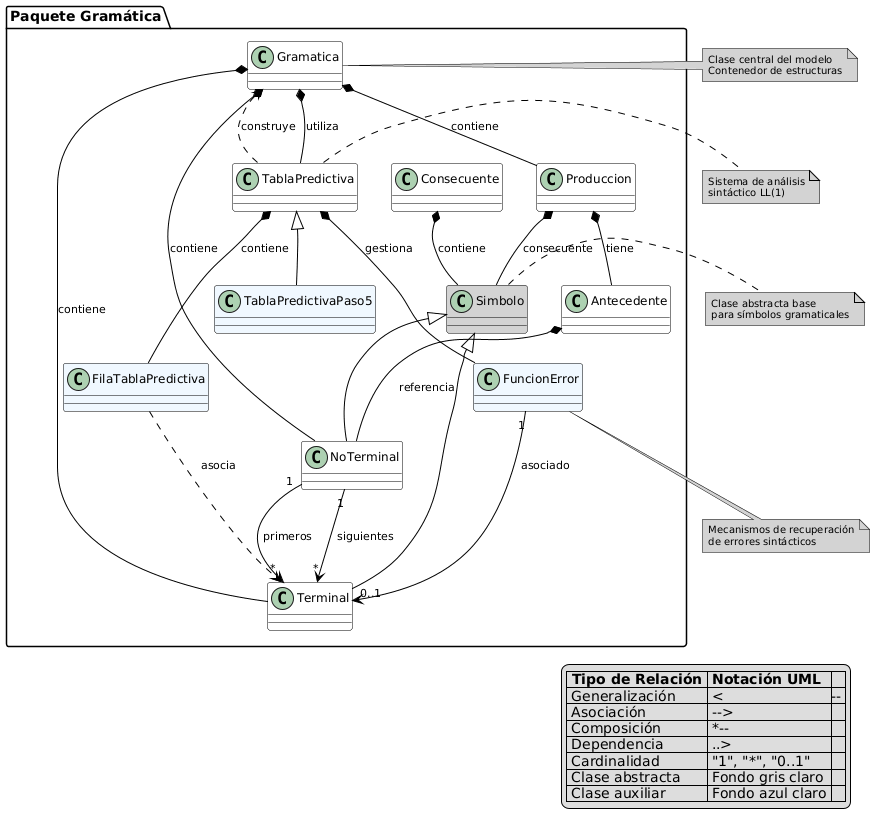
\includegraphics[width=0.9\textwidth]{figuras/Cap9/diagrama_gramatica_bueno.png}
    \caption{Diagrama de clases del paquete gramática - SimAS 3.0}
    \label{fig:diagrama_gramatica}
\end{figure}

\subsubsection{Patrones de diseño en el paquete gramática}

\begin{itemize}
    \item \textbf{Composite}: el patrón Composite se utiliza en la jerarquía de símbolos (Simbolo como componente base, Terminal y NoTerminal como componentes especializados) \cite{gamma1995design}.
    \item \textbf{Observer/Observable}: implementado mediante JavaFX Properties para notificación automática de cambios en la interfaz cuando se modifican los datos del modelo \cite{gamma1995design}.
    \item \textbf{Strategy}: el patrón Strategy se utiliza en las funciones de error (FuncionError) que encapsulan diferentes estrategias de recuperación de errores durante el análisis sintáctico \cite{gamma1995design}.
    \item \textbf{Factory Method}: utilizado en los constructores de TablaPredictiva y TablaPredictivaPaso5 para crear instancias con diferentes configuraciones \cite{gamma1995design}.
    \item \textbf{Builder}: implícito en la construcción de Gramatica a través de sus múltiples constructores que permiten diferentes configuraciones iniciales \cite{gamma1995design}.
    \item \textbf{Template Method}: utilizado en TablaPredictivaPaso5 que redefine métodos de TablaPredictiva para proporcionar comportamiento específico \cite{gamma1995design}.
    \item \textbf{MVC (Model-View-Controller)}: el paquete completo sigue el patrón MVC donde las clases del paquete gramática representan el Modelo, las clases de vistas manejan la presentación, y los controladores coordinan la interacción \cite{burbeck1992applications}.
\end{itemize}

\subsection{Paquete utils}

El paquete \textbf{utils} contiene las clases de utilidad transversales que proporcionan funcionalidades comunes y servicios compartidos utilizados por todos los demás paquetes de SimAS 3.0. Este paquete implementa servicios transversales como gestión de pestañas, internacionalización, monitoreo de componentes y gestión de ventanas secundarias.

Las clases de este paquete permiten:
\begin{itemize}
    \item Gestión avanzada de pestañas y navegación entre ventanas
    \item Sistema completo de internacionalización con soporte multiidioma
    \item Monitoreo y supervisión automática de componentes de la interfaz
    \item Gestión de ventanas secundarias y comunicación entre ellas
    \item Utilidades comunes para todas las capas de la aplicación
\end{itemize}

\subsubsection{Clases del paquete utils}

Este paquete contiene 6 clases principales que proporcionan servicios transversales a toda la aplicación SimAS 3.0, organizadas por funcionalidad: gestión de pestañas, internacionalización, monitoreo y ventanas. Además incluye archivos de propiedades para la internacionalización.

\subsubsection{Clase ActualizableTextos}

La clase \textbf{ActualizableTextos} es una interfaz que define el contrato para la actualización dinámica de textos en la interfaz de usuario cuando cambia el idioma de la aplicación.

\begin{longtable}[H]{|>{\columncolor[rgb]{0.63,0.79,0.95}}m{6cm} | m{8.5cm} |}
\caption{Clase ActualizableTextos - Interfaz de internacionalización}
\endfirsthead
\multicolumn{2}{c}{{\tablename\ \thetable{} -- continúa de la página anterior}} \\
\endhead
\hline \multicolumn{2}{|r|}{{Continúa en la página siguiente}} \\ \hline
\endfoot
\hline
\endlastfoot
\hline
\textbf{Nombre} & \textbf{ActualizableTextos} \\ \hline
\textbf{Descripción} & Interfaz que define el contrato para actualizar textos de la interfaz cuando cambia el idioma, implementada por todas las clases de UI que requieren internacionalización. \\ \hline
\textbf{Métodos} &
\begin{enumerate}
    \item \textbf{actualizarTextos(ResourceBundle)}: método que debe implementar cada clase para actualizar sus textos según el ResourceBundle proporcionado.
\end{enumerate}
\label{tabla_actualizable_textos}
\end{longtable}

\subsubsection{Clase LanguageItem}

La clase \textbf{LanguageItem} representa un elemento de idioma en el sistema de internacionalización, conteniendo información sobre el nombre del idioma, código de localización y bandera correspondiente.

\begin{longtable}[H]{|>{\columncolor[rgb]{0.63,0.79,0.95}}m{6cm} | m{8.5cm} |}
\caption{Clase LanguageItem - Elemento de idioma}
\endfirsthead
\multicolumn{2}{c}{{\tablename\ \thetable{} -- continúa de la página anterior}} \\
\endhead
\hline \multicolumn{2}{|r|}{{Continúa en la página siguiente}} \\ \hline
\endfoot
\hline
\endlastfoot
\hline
\textbf{Nombre} & \textbf{LanguageItem} \\ \hline
\textbf{Descripción} & Representa un idioma disponible en la aplicación, incluyendo su nombre, código de localización y bandera visual para el selector de idiomas. \\ \hline
\textbf{Atributos} &
\begin{enumerate}
    \item \textbf{name}: String con el nombre del idioma (ej: \string"Español\string", \string"English\string").
    \item \textbf{locale}: String con el código de localización (ej: \string"es\string", \string"en\string").
    \item \textbf{flagPath}: String con la ruta de la imagen de la bandera.
    \item \textbf{flagImageView}: ImageView que contiene la bandera visual del idioma.
\end{enumerate} \\ \hline
\textbf{Métodos} &
\begin{enumerate}
    \item \textbf{LanguageItem(String, String, String)}: constructor que inicializa el idioma con nombre, localización y ruta de bandera.
    \item \textbf{getName()}: obtiene el nombre del idioma.
    \item \textbf{getLocale()}: obtiene el código de localización.
    \item \textbf{getFlagPath()}: obtiene la ruta de la bandera.
    \item \textbf{getFlagImageView()}: obtiene el ImageView de la bandera.
    \item \textbf{toString()}: devuelve el nombre del idioma como representación textual.
    \item \textbf{equals(Object)}: compara dos LanguageItem por su código de localización.
    \item \textbf{hashCode()}: devuelve el hashCode basado en el código de localización.
\end{enumerate}
\label{tabla_language_item}
\end{longtable}

\subsubsection{Clase LanguageListCell}

La clase \textbf{LanguageListCell} es una celda personalizada para listas de selección de idiomas, que muestra la bandera y nombre del idioma de forma visual.

\begin{longtable}[H]{|>{\columncolor[rgb]{0.63,0.79,0.95}}m{6cm} | m{8.5cm} |}
\caption{Clase LanguageListCell - Celda de lista de idiomas}
\endfirsthead
\multicolumn{2}{c}{{\tablename\ \thetable{} -- continúa de la página anterior}} \\
\endhead
\hline \multicolumn{2}{|r|}{{Continúa en la página siguiente}} \\ \hline
\endfoot
\hline
\endlastfoot
\hline
\textbf{Nombre} & \textbf{LanguageListCell} \\ \hline
\textbf{Descripción} & Celda personalizada para ComboBox y ListView que muestra elementos de idioma con su bandera y nombre de forma visual. \\ \hline
\textbf{Atributos} &
\begin{enumerate}
    \item \textbf{Componentes FXML}: elementos de la interfaz para mostrar bandera y texto.
\end{enumerate} \\ \hline
\textbf{Métodos} &
\begin{enumerate}
    \item \textbf{LanguageListCell()}: constructor que inicializa la celda personalizada con componentes visuales.
    \item \textbf{updateItem(LanguageItem, boolean)}: actualiza el contenido visual de la celda con el idioma correspondiente, incluyendo bandera y texto.
\end{enumerate}
\label{tabla_language_list_cell}
\end{longtable}

\subsubsection{Clase TabManager}

La clase \textbf{TabManager} es el gestor central de pestañas de la aplicación, responsable de crear, gestionar y coordinar todas las pestañas en múltiples ventanas.

\begin{longtable}[H]{|>{\columncolor[rgb]{0.63,0.79,0.95}}m{6cm} | m{8.5cm} |}
\caption{Clase TabManager - Gestor central de pestañas}
\endfirsthead
\multicolumn{2}{c}{{\tablename\ \thetable{} -- continúa de la página anterior}} \\
\endhead
\hline \multicolumn{2}{|r|}{{Continúa en la página siguiente}} \\ \hline
\endfoot
\hline
\endlastfoot
\hline
\textbf{Nombre} & \textbf{TabManager} \\ \hline
\textbf{Descripción} & Gestor central que maneja la creación, gestión y coordinación de todas las pestañas en la aplicación, incluyendo relaciones padre-hijo y grupos de gramáticas. \\ \hline
\textbf{Atributos} &
\begin{enumerate}
    \item \textbf{tabInstances}: Map que almacena instancias de pestañas por TabPane y tipo.
    \item \textbf{parentChildRelations}: Map que mantiene las relaciones padre-hijo entre pestañas.
    \item \textbf{elementoToGrupo}: Map que asocia elementos con sus grupos de gramática.
    \item \textbf{gruposGramatica}: Map que contiene los números de grupo para cada grupo.
    \item \textbf{resourceBundles}: Map que almacena ResourceBundles por TabPane.
    \item \textbf{contadorGrupos}: contador global para generar IDs únicos de grupo.
\end{enumerate} \\ \hline
\textbf{Métodos} &
\begin{enumerate}
    \item \textbf{getOrCreateTab(TabPane, Class, String, Object)}: obtiene o crea una pestaña del tipo especificado.
    \item \textbf{getOrCreateTab(TabPane, Class, String, Object, String, String)}: versión completa con IDs padre-hijo.
    \item \textbf{asignarElementoANuevoGrupo( TabPane, String)}: asigna un elemento a un nuevo grupo de gramática.
    \item \textbf{contarGruposActivos(TabPane)}: cuenta los grupos activos en un TabPane.
    \item \textbf{isSimuladorContent(Object)}: verifica si un objeto es contenido de simulador.
    \item \textbf{isSimuladorTab(Tab)}: verifica si una pestaña es de simulador.
    \item \textbf{obtenerGrupoDeElemento(TabPane, String)}: obtiene el grupo al que pertenece un elemento.
    \item \textbf{asignarSimuladorAGrupoDeEditor( TabPane, String, String)}: asigna un simulador al grupo de un editor.
    \item \textbf{calcularPosicionInsercion(TabPane, Class, String, String)}: calcula la posición de inserción de una nueva pestaña.
    \item \textbf{calcularPosicionSeguaDespues DelMenu(TabPane)}: calcula posición segura después del menú.
    \item \textbf{isPestañaHijaDeElemento(String, String)}: verifica si una pestaña es hija de un elemento.
    \item \textbf{isEditorContent(Object)}: verifica si un objeto es contenido de editor.
    \item \textbf{closeTab(TabPane, Class)}: cierra una pestaña específica.
    \item \textbf{hasTab(TabPane, Class)}: verifica si existe una pestaña de cierto tipo.
    \item \textbf{closeChildTabs(TabPane, String)}: cierra todas las pestañas hijas de un elemento.
    \item \textbf{closeAllDescendantTabs(TabPane, String)}: cierra todos los descendientes de un elemento.
    \item \textbf{reasignarNumerosGruposGramatica(TabPane)}: reasigna números de grupo después de cambios.
    \item \textbf{setResourceBundle(TabPane, ResourceBundle)}: establece el ResourceBundle para un TabPane.
    \item \textbf{obtenerNumeroGrupo(TabPane, String)}: obtiene el número de grupo de un elemento.
    \item \textbf{eliminarElementoDeGrupo(TabPane, String, String)}: elimina un elemento de un grupo.
    \item \textbf{resetGrupos(TabPane)}: resetea todos los grupos de un TabPane.
    \item \textbf{asignarElementoAGrupo(TabPane, String, String)}: asigna un elemento a un grupo específico.
    \item \textbf{configurarMenuContextual(TabPane, ResourceBundle)}: configura el menú contextual de las pestañas.
    \item \textbf{actualizarMenuContextual(TabPane, ResourceBundle)}: actualiza el menú contextual con nuevos textos.
    \item \textbf{actualizarIdsRelacionados(TabPane, String, String)}: actualiza IDs relacionados de un simulador.
    \item \textbf{actualizarTitulosPestañas(TabPane)}: actualiza los títulos de todas las pestañas.
    \item \textbf{debugTabPaneState(TabPane)}: imprime el estado del TabPane para debugging.
    \item \textbf{moverGrupoEntreVentanasMejorado(TabPane, TabPane, String, Tab)}: mueve un grupo entre ventanas.
    \item \textbf{getElementoToGrupo(TabPane)}: obtiene el mapa de elementos a grupos.
    \item \textbf{getGruposGramatica(TabPane)}: obtiene el mapa de grupos de gramática.
\end{enumerate}
\label{tabla_tab_manager}
\end{longtable}

\subsubsection{Clase TabPaneMonitor}

La clase \textbf{TabPaneMonitor} es un monitor singleton que supervisa continuamente el estado de todos los TabPane activos en la aplicación, validando consistencia y reparando automáticamente inconsistencias.

\begin{longtable}[H]{|>{\columncolor[rgb]{0.63,0.79,0.95}}m{6cm} | m{8.5cm} |}
\caption{Clase TabPaneMonitor - Monitor de pestañas}
\endfirsthead
\multicolumn{2}{c}{{\tablename\ \thetable{} -- continúa de la página anterior}} \\
\endhead
\hline \multicolumn{2}{|r|}{{Continúa en la página siguiente}} \\ \hline
\endfoot
\hline
\endlastfoot
\hline
\textbf{Nombre} & \textbf{TabPaneMonitor} \\ \hline
\textbf{Descripción} & Monitor singleton que supervisa continuamente todos los TabPanes activos, validando la consistencia de grupos y relaciones padre-hijo, y reparando automáticamente las inconsistencias detectadas. \\ \hline
\textbf{Atributos} &
\begin{enumerate}
    \item \textbf{instance}: instancia singleton del monitor.
    \item \textbf{monitoredTabPanes}: Map que contiene los TabPanes monitoreados.
    \item \textbf{scheduler}: ScheduledExecutorService para monitoreo periódico.
    \item \textbf{debugMode}: boolean que indica si está en modo debug.
    \item \textbf{movimientoEnProgreso}: boolean que indica si hay un movimiento en progreso.
    \item \textbf{contadorReparaciones}: Map que cuenta las reparaciones por TabPane.
\end{enumerate} \\ \hline
\textbf{Métodos} &
\begin{enumerate}
    \item \textbf{getInstance()}: obtiene la instancia singleton del monitor.
    \item \textbf{registrarTabPane(TabPane, String)}: registra un TabPane para monitoreo.
    \item \textbf{desregistrarTabPane(TabPane)}: desregistra un TabPane del monitoreo.
    \item \textbf{validarConsistenciaTabPane( TabPane, boolean)}: valida la consistencia de un TabPane específico.
    \item \textbf{forzarValidacion(TabPane)}: fuerza una validación inmediata de un TabPane.
    \item \textbf{obtenerEstadisticas()}: obtiene estadísticas del monitoreo.
    \item \textbf{shutdown()}: detiene el monitoreo y libera recursos.
    \item \textbf{setMovimientoEnProgreso(boolean)}: establece si hay un movimiento en progreso.
    \item \textbf{reiniciarContadorReparaciones( TabPane)}: reinicia el contador de reparaciones de un TabPane.
    \item \textbf{reiniciarTodosLosContadores()}: reinicia todos los contadores de reparaciones.
\end{enumerate} \\ \hline
\textbf{Clase Interna TabPaneInfo} &
\begin{enumerate}
    \item \textbf{TabPaneInfo(TabPane, String)}: constructor de la información de TabPane.
    \item \textbf{tabPane}: referencia al TabPane monitoreado.
    \item \textbf{tabChangeListener}: listener para cambios en pestañas.
    \item \textbf{identifier}: identificador único del TabPane.
    \item \textbf{lastValidation}: timestamp de la última validación.
    \item \textbf{lastKnownGroups}: último estado conocido de grupos.
    \item \textbf{lastKnownRelations}: último estado conocido de relaciones.
\end{enumerate}
\label{tabla_tab_pane_monitor}
\end{longtable}

\subsubsection{Clase SecondaryWindow}

La clase \textbf{SecondaryWindow} extiende EditorWindow para crear ventanas secundarias que permiten trabajar con pestañas de forma independiente de la ventana principal.

\begin{longtable}[H]{|>{\columncolor[rgb]{0.63,0.79,0.95}}m{6cm} | m{8.5cm} |}
\caption{Clase SecondaryWindow - Ventanas secundarias}
\endfirsthead
\multicolumn{2}{c}{{\tablename\ \thetable{} -- continúa de la página anterior}} \\
\endhead
\hline \multicolumn{2}{|r|}{{Continúa en la página siguiente}} \\ \hline
\endfoot
\hline
\endlastfoot
\hline
\textbf{Nombre} & \textbf{SecondaryWindow} \\ \hline
\textbf{Descripción} & Extiende EditorWindow para crear ventanas secundarias que permiten trabajar con pestañas de forma independiente, facilitando la organización del espacio de trabajo. \\ \hline
\textbf{Atributos} &
\begin{enumerate}
    \item \textbf{activeWindows}: Map estático que mantiene todas las ventanas secundarias activas.
    \item \textbf{windowId}: identificador único de la ventana secundaria.
    \item \textbf{localTabPane}: TabPane específico de esta ventana secundaria.
    \item \textbf{stage}: Stage de la ventana secundaria.
    \item \textbf{bundle}: ResourceBundle para internacionalización.
    \item \textbf{windowNumber}: número secuencial de la ventana.
\end{enumerate} \\ \hline
\textbf{Métodos} &
\begin{enumerate}
    \item \textbf{SecondaryWindow(ResourceBundle, String)}: constructor que inicializa la ventana secundaria.
    \item \textbf{getActiveWindows()}: obtiene un mapa con todas las ventanas secundarias activas.
    \item \textbf{moveGroupToWindow(TabPane, String, Tab)}: mueve un grupo de pestañas a esta ventana.
    \item \textbf{show()}: muestra la ventana secundaria.
    \item \textbf{getTabPane()}: obtiene el TabPane de la ventana secundaria.
    \item \textbf{addTab(Tab)}: añade una pestaña individual a la ventana.
    \item \textbf{getStage()}: obtiene el Stage de la ventana secundaria.
    \item \textbf{actualizarIdioma(ResourceBundle)}: actualiza el idioma de la ventana secundaria.
    \item \textbf{getWindowNumber()}: obtiene el número de la ventana.
\end{enumerate} \\ \hline
\textbf{Métodos Estáticos} &
\begin{enumerate}
    \item \textbf{getActiveWindows()}: obtiene todas las ventanas secundarias activas.
    \item \textbf{getActiveWindowCount()}: obtiene el conteo de ventanas secundarias activas.
\end{enumerate}
\label{tabla_secondary_window}
\end{longtable}

\subsubsection{Dependencias internas del paquete utils}

Las dependencias internas del paquete utils se ilustran en la Figura \ref{fig:diagrama_utils}, donde se puede apreciar la estructura organizada de servicios transversales que proporciona este paquete.

\begin{itemize}
    \item \textbf{TabManager $\leftrightarrow$ TabPaneMonitor}: TabManager utiliza TabPaneMonitor para supervisar los TabPane que gestiona.
    \item \textbf{SecondaryWindow $\rightarrow$ EditorWindow}: SecondaryWindow extiende EditorWindow para crear ventanas independientes.
    \item \textbf{SecondaryWindow $\rightarrow$ TabManager}: SecondaryWindow utiliza TabManager para gestionar sus pestañas.
    \item \textbf{LanguageItem $\leftrightarrow$ LanguageListCell}: LanguageListCell utiliza LanguageItem para mostrar idiomas en listas.
    \item \textbf{ActualizableTextos $\leftarrow$ (todas las clases de UI)}: interfaz implementada por todas las clases que requieren internacionalización.
    \item \textbf{TabManager $\leftrightarrow$ SecondaryWindow}: comunicación bidireccional para gestión de pestañas entre ventanas.
    \item \textbf{Archivos .properties}: todos los archivos de propiedades de idiomas son utilizados por el sistema de internacionalización.
\end{itemize}

\begin{figure}[H]
    \centering
    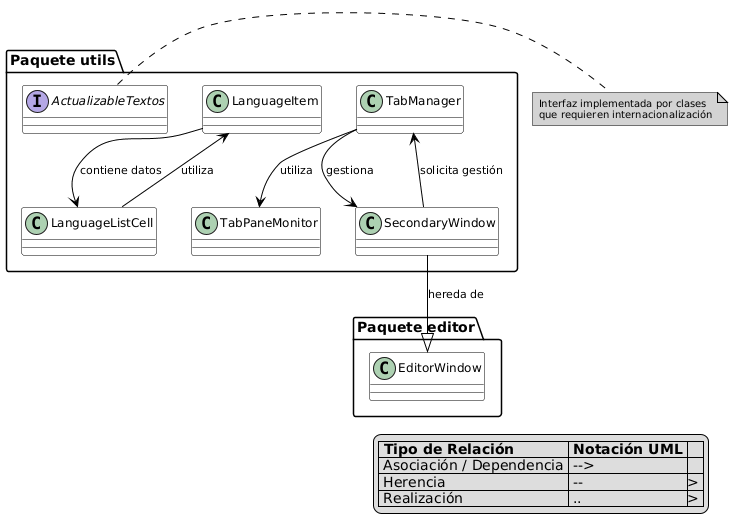
\includegraphics[width=0.9\textwidth]{figuras/Cap9/diagrama_utils.png}
    \caption{Diagrama de dependencias del paquete utils - SimAS 3.0}
    \label{fig:diagrama_utils}
\end{figure}

\subsubsection{Patrones de diseño en el paquete utils}

\begin{itemize}
    \item \textbf{Singleton}: implementado en TabPaneMonitor para asegurar una única instancia que supervise toda la aplicación \cite{gamma1995design}.
    \item \textbf{Observer}: utilizado en TabPaneMonitor para observar cambios en los TabPane y reaccionar automáticamente \cite{gamma1995design}.
    \item \textbf{Facade}: TabManager actúa como fachada que simplifica la gestión compleja de pestañas y relaciones \cite{gamma1995design}.
    \item \textbf{Factory Method}: implícito en los constructores de TabManager para crear diferentes tipos de pestañas \cite{gamma1995design}.
    \item \textbf{Monitor Object}: TabPaneMonitor implementa el patrón Monitor Object para sincronización segura de acceso a recursos compartidos.
    \item \textbf{Registry}: SecondaryWindow utiliza un registro estático para mantener todas las ventanas secundarias activas.
\end{itemize}

\subsection{Paquete editor}

El paquete \textbf{editor} contiene las clases responsables de la interfaz de usuario para la creación y edición de gramáticas de contexto libre en SimAS 3.0. Este paquete implementa el patrón de diseño MVC donde las clases del editor actúan como controladores que coordinan la interacción entre la vista (componentes JavaFX) y el modelo (paquete gramática).

Las clases de este paquete permiten:
\begin{itemize}
    \item Crear gramáticas mediante un asistente paso a paso
    \item Editar símbolos terminales y no terminales
    \item Gestionar producciones gramaticales
    \item Validar gramáticas creadas
    \item Gestionar múltiples editores en pestañas
    \item Integración completa con el sistema de internacionalización
\end{itemize}

\subsubsection{Clases del paquete editor}

Este paquete contiene 10 clases principales que conforman la interfaz de edición de SimAS 3.0, organizadas jerárquicamente desde la gestión de ventanas hasta los componentes específicos de edición.

\subsubsection{Clase EditorWindow}

La clase \textbf{EditorWindow} representa la ventana principal del editor de gramáticas, gestionando el ciclo de vida de la aplicación de edición y coordinando múltiples pestañas de edición.

\begin{longtable}[H]{|>{\columncolor[rgb]{0.63,0.79,0.95}}m{6cm} | m{8.5cm} |}
\caption{Clase EditorWindow - Ventana principal del editor}
\endfirsthead
\multicolumn{2}{c}{{\tablename\ \thetable{} -- continúa de la página anterior}} \\
\endhead
\hline \multicolumn{2}{|r|}{{Continúa en la página siguiente}} \\ \hline
\endfoot
\hline
\endlastfoot
\hline
\textbf{Nombre} & \textbf{EditorWindow} \\ \hline
\textbf{Descripción} & Gestiona la ventana principal del editor, incluyendo el sistema de pestañas, atajos de teclado y funcionalidades de arrastrar y soltar. \\ \hline
\textbf{Atributos} &
\begin{enumerate}
    \item \textbf{stage}: Stage principal de la ventana del editor.
    \item \textbf{tabPane}: TabPane que contiene todas las pestañas de edición.
    \item \textbf{bundle}: ResourceBundle para internacionalización.
\end{enumerate} \\ \hline
\textbf{Métodos} &
\begin{enumerate}
    \item \textbf{EditorWindow(ResourceBundle)}: constructor que inicializa la ventana con internacionalización.
    \item \textbf{initialize()}: configura la ventana, escena y componentes principales.
    \item \textbf{configurarAtajosTeclado(Scene)}: establece los atajos de teclado globales.
    \item \textbf{findFirstTabInGroup(int)}: encuentra la primera pestaña de un grupo específico.
    \item \textbf{show()}: muestra la ventana del editor.
    \item \textbf{addTab(Tab)}: añade una pestaña a la ventana.
    \item \textbf{moveGroupToWindow(TabPane, String, Tab)}: mueve un grupo de pestañas a esta ventana.
    \item \textbf{addEditor(Editor)}: añade un editor como nueva pestaña.
    \item \textbf{getTabPane()}: obtiene el TabPane de la ventana.
    \item \textbf{abrirEditorEnEditorWindow()}: abre un nuevo editor en esta ventana.
    \item \textbf{abrirSimuladorEnEditorWindow()}: abre el simulador directo en esta ventana.
    \item \textbf{cargarGramaticaYSimular DirectamenteEnEditorWindow()}: carga gramática y va directo a simulación.
    \item \textbf{crearSimuladorDirectoAl Paso6EnEditorWindow( Gramatica)}: crea simulador directo al paso 6.
    \item \textbf{abrirAyuda()}: abre el manual de ayuda.
    \item \textbf{abrirTutorial()}: abre el tutorial.
    \item \textbf{salirAplicacion()}: sale de la aplicación.
    \item \textbf{mostrarErroresValidacion( ObservableList<String>)}: muestra errores de validación.
    \item \textbf{mostrarError(String, String)}: muestra mensaje de error simple.
\end{enumerate}
\label{tabla_editor_window}
\end{longtable}

\subsubsection{Clase Editor}

La clase \textbf{Editor} representa la interfaz principal de edición de una gramática específica, proporcionando acceso a todas las funcionalidades de edición y gestión.

\begin{longtable}[H]{|>{\columncolor[rgb]{0.63,0.79,0.95}}m{6cm} | m{8.5cm} |}
\caption{Clase Editor - Interfaz principal de edición}
\endfirsthead
\multicolumn{2}{c}{{\tablename\ \thetable{} -- continúa de la página anterior}} \\
\endhead
\hline \multicolumn{2}{|r|}{{Continúa en la página siguiente}} \\ \hline
\endfoot
\hline
\endlastfoot
\hline
\textbf{Nombre} & \textbf{Editor} \\ \hline
\textbf{Descripción} & Clase principal que representa un editor de gramáticas, gestionando la interfaz de usuario y la coordinación con el modelo de datos. \\ \hline
\textbf{Atributos} &
\begin{enumerate}
    \item \textbf{gramatica}: instancia de Gramatica que se está editando.
    \item \textbf{tabPane}: referencia al TabPane contenedor.
    \item \textbf{menuPane}: referencia al MenuPrincipal.
    \item \textbf{bundle}: ResourceBundle para internacionalización.
    \item \textbf{editorId}: identificador único del editor.
    \item \textbf{rootPane}: BorderPane raíz de la interfaz.
    \item \textbf{Componentes FXML}: botones, campos de texto, listas, etiquetas.
\end{enumerate} \\ \hline
\textbf{Métodos} &
\begin{enumerate}
    \item \textbf{Editor()}: constructor vacío para carga FXML.
    \item \textbf{Editor(TabPane, MenuPrincipal)}: constructor con TabPane y MenuPrincipal.
    \item \textbf{Editor(TabPane, Gramatica, MenuPrincipal)}: constructor con gramática preexistente.
    \item \textbf{Editor(TabPane, MenuPrincipal, ResourceBundle)}: constructor con internacionalización.
    \item \textbf{configurarRelacionesPadreHijo()}: configura las relaciones padre-hijo para cerrar pestañas hijas.
    \item \textbf{cargarFXML()}: carga la interfaz desde archivo FXML.
    \item \textbf{getEditorId()}: obtiene el ID único del editor.
    \item \textbf{getGramatica()}: obtiene la gramática actual.
    \item \textbf{setGramatica(Gramatica)}: establece una nueva gramática.
    \item \textbf{initialize()}: método de inicialización FXML.
    \item \textbf{setTabPane(TabPane)}: establece la referencia al TabPane.
    \item \textbf{setMenuPane(MenuPrincipal)}: establece la referencia al MenuPrincipal.
    \item \textbf{getRoot()}: obtiene el componente raíz.
    \item \textbf{cargarGramatica()}: carga una gramática desde archivo.
    \item \textbf{grabarGramatica()}: guarda la gramática actual.
    \item \textbf{actualizarVisualizacion()}: actualiza la visualización de los datos.
    \item \textbf{validarGramatica(Gramatica)}: valida una gramática específica.
    \item \textbf{actualizarTextos(ResourceBundle)}: actualiza textos para internacionalización.
    \item \textbf{getBundle()}: obtiene el ResourceBundle.
    \item \textbf{setBundle(ResourceBundle)}: establece el ResourceBundle.
\end{enumerate}
\label{tabla_editor}
\end{longtable}

\subsubsection{Clase PanelCreacionGramatica}

La clase \textbf{PanelCreacionGramatica} coordina el asistente de creación de gramáticas paso a paso, gestionando la navegación entre los diferentes pasos del proceso.

\begin{longtable}[H]{|>{\columncolor[rgb]{0.63,0.79,0.95}}m{6cm} | m{8.5cm} |}
\caption{Clase PanelCreacionGramatica - Asistente de creación}
\endfirsthead
\multicolumn{2}{c}{{\tablename\ \thetable{} -- continúa de la página anterior}} \\
\endhead
\hline \multicolumn{2}{|r|}{{Continúa en la página siguiente}} \\ \hline
\endfoot
\hline
\endlastfoot
\hline
\textbf{Nombre} & \textbf{PanelCreacionGramatica} \\ \hline
\textbf{Descripción} & Coordina el asistente paso a paso para la creación de gramáticas, gestionando la navegación y el flujo de datos entre los diferentes paneles. \\ \hline
\textbf{Atributos} &
\begin{enumerate}
    \item \textbf{tabPane}: TabPane contenedor de las pestañas.
    \item \textbf{paso1-4}: instancias de los paneles de cada paso del asistente.
    \item \textbf{panelPadre}: referencia al Editor padre.
    \item \textbf{menuPane}: referencia al MenuPrincipal.
    \item \textbf{gramaticaTemporal}: copia temporal de la gramática en edición.
    \item \textbf{bundle}: ResourceBundle para internacionalización.
    \item \textbf{creacionId}: identificador único del proceso de creación.
\end{enumerate} \\ \hline
\textbf{Métodos} &
\begin{enumerate}
    \item \textbf{PanelCreacionGramatica(Editor, TabPane, Gramatica, MenuPrincipal)}: constructor principal.
    \item \textbf{PanelCreacionGramatica(Editor, TabPane, Gramatica, MenuPrincipal, String)}: constructor con ID específico.
    \item \textbf{configurarRelacionesPadreHijo()}: configura las relaciones padre-hijo.
    \item \textbf{getCreacionId()}: obtiene el ID único del proceso de creación.
    \item \textbf{getGramatica()}: obtiene la gramática temporal.
    \item \textbf{setGramatica(Gramatica)}: establece la gramática temporal.
    \item \textbf{cambiarPaso(int)}: cambia al paso especificado.
    \item \textbf{getMenuPane()}: obtiene la referencia al MenuPrincipal.
    \item \textbf{getPanelPadre()}: obtiene la referencia al Editor padre.
    \item \textbf{cancelarEdicion()}: cancela la edición actual.
    \item \textbf{mostrarAlerta(String, String)}: muestra una alerta al usuario.
    \item \textbf{actualizarTextos(ResourceBundle)}: actualiza textos para internacionalización.
    \item \textbf{getBundle()}: obtiene el ResourceBundle.
\end{enumerate}
\label{tabla_panel_creacion_gramatica}
\end{longtable}

\subsubsection{Clase PanelCreacionGramaticaPaso1}

La clase \textbf{PanelCreacionGramaticaPaso1} maneja el primer paso del asistente de creación, donde se definen los metadatos básicos de la gramática.

\begin{longtable}[H]{|>{\columncolor[rgb]{0.63,0.79,0.95}}m{6cm} | m{8.5cm} |}
\caption{Clase PanelCreacionGramaticaPaso1 - Paso 1: Metadatos}
\endfirsthead
\multicolumn{2}{c}{{\tablename\ \thetable{} -- continúa de la página anterior}} \\
\endhead
\hline \multicolumn{2}{|r|}{{Continúa en la página siguiente}} \\ \hline
\endfoot
\hline
\endlastfoot
\hline
\textbf{Nombre} & \textbf{PanelCreacionGramaticaPaso1} \\ \hline
\textbf{Descripción} & Primer paso del asistente de creación de gramáticas, donde se definen el nombre, descripción y símbolo inicial. \\ \hline
\textbf{Atributos} &
\begin{enumerate}
    \item \textbf{panelPadre}: referencia al PanelCreacionGramatica padre.
    \item \textbf{bundle}: ResourceBundle para internacionalización.
    \item \textbf{Componentes FXML}: campos de texto para nombre, descripción y símbolo inicial.
    \item \textbf{btnSiguiente}: botón para avanzar al siguiente paso.
    \item \textbf{btnCancelar}: botón para cancelar la creación.
\end{enumerate} \\ \hline
\textbf{Métodos} &
\begin{enumerate}
    \item \textbf{PanelCreacionGramaticaPaso1( PanelCreacionGramatica, ResourceBundle)}: constructor.
    \item \textbf{cargarFXML()}: carga la interfaz desde archivo FXML.
    \item \textbf{initialize()}: método de inicialización FXML.
    \item \textbf{configurarValidaciones()}: configura las validaciones en tiempo real.
    \item \textbf{setNombre(String)}: establece el nombre de la gramática.
    \item \textbf{setDescripcion(String)}: establece la descripción de la gramática.
    \item \textbf{actualizarTextos(ResourceBundle)}: actualiza textos para internacionalización.
\end{enumerate}
\label{tabla_panel_creacion_paso1}
\end{longtable}

\subsubsection{Clase PanelCreacionGramaticaPaso2}

La clase \textbf{PanelCreacionGramaticaPaso2} maneja el segundo paso del asistente de creación, donde se definen los símbolos terminales y no terminales.

\begin{longtable}[H]{|>{\columncolor[rgb]{0.63,0.79,0.95}}m{6cm} | m{8.5cm} |}
\caption{Clase PanelCreacionGramaticaPaso2 - Paso 2: Símbolos}
\endfirsthead
\multicolumn{2}{c}{{\tablename\ \thetable{} -- continúa de la página anterior}} \\
\endhead
\hline \multicolumn{2}{|r|}{{Continúa en la página siguiente}} \\ \hline
\endfoot
\hline
\endlastfoot
\hline
\textbf{Nombre} & \textbf{PanelCreacionGramaticaPaso2} \\ \hline
\textbf{Descripción} & Segundo paso del asistente donde se definen y gestionan los símbolos terminales y no terminales de la gramática. \\ \hline
\textbf{Atributos} &
\begin{enumerate}
    \item \textbf{panelPadre}: referencia al PanelCreacionGramatica padre.
    \item \textbf{menuPane}: referencia al MenuPrincipal.
    \item \textbf{tabPane}: TabPane para gestión de pestañas.
    \item \textbf{panelTerminales}: PanelSimbolosTerminales para gestión de terminales.
    \item \textbf{panelNoTerminales}: PanelSimbolosNoTerminales para gestión de no terminales.
    \item \textbf{bundle}: ResourceBundle para internacionalización.
    \item \textbf{btnSiguiente, btnAnterior, btnCancelar}: botones de navegación.
\end{enumerate} \\ \hline
\textbf{Métodos} &
\begin{enumerate}
    \item \textbf{PanelCreacionGramaticaPaso2( PanelCreacionGramatica, MenuPrincipal, TabPane)}: constructor.
    \item \textbf{cargarFXML()}: carga la interfaz desde archivo FXML.
    \item \textbf{initialize()}: método de inicialización FXML.
    \item \textbf{aplicarEstilosResponsivos()}: aplica estilos responsivos según el tamaño de pantalla.
    \item \textbf{cargarDatosDesdeGramatica()}: carga datos desde la gramática padre.
    \item \textbf{configurarValidacionSimbolos()}: configura la validación de símbolos.
    \item \textbf{asignarListaSimbolosNoTerminales( ObservableList<String>)}: asigna la lista de no terminales.
    \item \textbf{asignarListaSimbolosTerminales( ObservableList<String>)}: asigna la lista de terminales.
    \item \textbf{actualizarTextos(ResourceBundle)}: actualiza textos para internacionalización.
\end{enumerate}
\label{tabla_panel_creacion_paso2}
\end{longtable}

\subsubsection{Clase PanelCreacionGramaticaPaso3}

La clase \textbf{PanelCreacionGramaticaPaso3} maneja el tercer paso del asistente, donde se definen las producciones de la gramática.

\begin{longtable}[H]{|>{\columncolor[rgb]{0.63,0.79,0.95}}m{6cm} | m{8.5cm} |}
\caption{Clase PanelCreacionGramaticaPaso3 - Paso 3: Producciones}
\endfirsthead
\multicolumn{2}{c}{{\tablename\ \thetable{} -- continúa de la página anterior}} \\
\endhead
\hline \multicolumn{2}{|r|}{{Continúa en la página siguiente}} \\ \hline
\endfoot
\hline
\endlastfoot
\hline
\textbf{Nombre} & \textbf{PanelCreacionGramaticaPaso3} \\ \hline
\textbf{Descripción} & Tercer paso del asistente donde se definen y gestionan las producciones de la gramática. \\ \hline
\textbf{Atributos} &
\begin{enumerate}
    \item \textbf{panelPadre}: referencia al PanelCreacionGramatica padre.
    \item \textbf{tabPane}: TabPane para gestión de pestañas.
    \item \textbf{menuPane}: referencia al MenuPrincipal.
    \item \textbf{panelProducciones}: PanelProducciones para gestión de producciones.
    \item \textbf{bundle}: ResourceBundle para internacionalización.
    \item \textbf{btnSiguiente, btnAnterior, btnCancelar}: botones de navegación.
\end{enumerate} \\ \hline
\textbf{Métodos} &
\begin{enumerate}
    \item \textbf{PanelCreacionGramaticaPaso3( PanelCreacionGramatica, TabPane, MenuPrincipal)}: constructor.
    \item \textbf{cargarFXML()}: carga la interfaz desde archivo FXML.
    \item \textbf{initialize()}: método de inicialización FXML.
    \item \textbf{asignarProducciones( ObservableList<Produccion>)}: asigna las producciones existentes.
    \item \textbf{configurarValidacionProducciones()}: configura la validación de producciones.
    \item \textbf{actualizarTextos(ResourceBundle)}: actualiza textos para internacionalización.
\end{enumerate}
\label{tabla_panel_creacion_paso3}
\end{longtable}

\subsubsection{Clase PanelCreacionGramaticaPaso4}

La clase \textbf{PanelCreacionGramaticaPaso4} maneja el cuarto y último paso del asistente, donde se realiza la validación final y se completa la creación.

\begin{longtable}[H]{|>{\columncolor[rgb]{0.63,0.79,0.95}}m{6cm} | m{8.5cm} |}
\caption{Clase PanelCreacionGramaticaPaso4 - Paso 4: Validación}
\endfirsthead
\multicolumn{2}{c}{{\tablename\ \thetable{} -- continúa de la página anterior}} \\
\endhead
\hline \multicolumn{2}{|r|}{{Continúa en la página siguiente}} \\ \hline
\endfoot
\hline
\endlastfoot
\hline
\textbf{Nombre} & \textbf{PanelCreacionGramaticaPaso4} \\ \hline
\textbf{Descripción} & Cuarto y último paso del asistente donde se elige el símbolo inicial y se finaliza el proceso de creación. \\ \hline
\textbf{Atributos} &
\begin{enumerate}
    \item \textbf{panelPadre}: referencia al PanelCreacionGramatica padre.
    \item \textbf{tabPane}: TabPane para gestión de pestañas.
    \item \textbf{bundle}: ResourceBundle para internacionalización.
    \item \textbf{Componentes FXML}: etiquetas, botones de finalizar y cancelar.
    \item \textbf{areaValidacion}: área de texto para mostrar resultados de validación.
\end{enumerate} \\ \hline
\textbf{Métodos} &
\begin{enumerate}
    \item \textbf{PanelCreacionGramaticaPaso4( PanelCreacionGramatica, TabPane)}: constructor.
    \item \textbf{cargarFXML()}: carga la interfaz desde archivo FXML.
    \item \textbf{initialize()}: método de inicialización FXML.
    \item \textbf{configurarValidacionSimboloInicial()}: configura la validación del símbolo inicial.
    \item \textbf{cerrarAsistente()}: cierra el asistente de creación.
    \item \textbf{actualizarTextos(ResourceBundle)}: actualiza textos para internacionalización.
\end{enumerate}
\label{tabla_panel_creacion_paso4}
\end{longtable}

\subsubsection{Clase PanelProducciones}

La clase \textbf{PanelProducciones} proporciona la interfaz para editar y gestionar las producciones de la gramática.

\begin{longtable}[H]{|>{\columncolor[rgb]{0.63,0.79,0.95}}m{6cm} | m{8.5cm} |}
\caption{Clase PanelProducciones - Gestión de producciones}
\endfirsthead
\multicolumn{2}{c}{{\tablename\ \thetable{} -- continúa de la página anterior}} \\
\endhead
\hline \multicolumn{2}{|r|}{{Continúa en la página siguiente}} \\ \hline
\endfoot
\hline
\endlastfoot
\hline
\textbf{Nombre} & \textbf{PanelProducciones} \\ \hline
\textbf{Descripción} & Panel especializado para la creación, edición y eliminación de producciones gramaticales. \\ \hline
\textbf{Atributos} &
\begin{enumerate}
    \item \textbf{panelPadre}: referencia al PanelCreacionGramaticaPaso3 padre.
    \item \textbf{tabPane}: TabPane para gestión de pestañas.
    \item \textbf{producciones}: ObservableList de producciones.
    \item \textbf{noTerminales}: ObservableList de símbolos no terminales disponibles.
    \item \textbf{terminales}: ObservableList de símbolos terminales disponibles.
    \item \textbf{bundle}: ResourceBundle para internacionalización.
    \item \textbf{Componentes FXML}: ComboBox, TextField, ListViews, Buttons, Labels.
\end{enumerate} \\ \hline
\textbf{Métodos} &
\begin{enumerate}
    \item \textbf{PanelProducciones( PanelCreacionGramaticaPaso3, ObservableList<Produccion>, TabPane)}: constructor.
    \item \textbf{cargarFXML()}: carga la interfaz desde archivo FXML.
    \item \textbf{initialize()}: método de inicialización FXML.
    \item \textbf{actualizarTextos(ResourceBundle)}: actualiza textos para internacionalización.
\end{enumerate}
\label{tabla_panel_producciones}
\end{longtable}

\subsubsection{Clase PanelSimbolosTerminales}

La clase \textbf{PanelSimbolosTerminales} proporciona la interfaz para gestionar los símbolos terminales de la gramática.

\begin{longtable}[H]{|>{\columncolor[rgb]{0.63,0.79,0.95}}m{6cm} | m{8.5cm} |}
\caption{Clase PanelSimbolosTerminales - Gestión de terminales}
\endfirsthead
\multicolumn{2}{c}{{\tablename\ \thetable{} -- continúa de la página anterior}} \\
\endhead
\hline \multicolumn{2}{|r|}{{Continúa en la página siguiente}} \\ \hline
\endfoot
\hline
\endlastfoot
\hline
\textbf{Nombre} & \textbf{PanelSimbolosTerminales} \\ \hline
\textbf{Descripción} & Panel especializado para la gestión de símbolos terminales, incluyendo símbolos predefinidos y personalizados. \\ \hline
\textbf{Atributos} &
\begin{enumerate}
    \item \textbf{panelPadre}: referencia al PanelCreacionGramaticaPaso2 padre.
    \item \textbf{tabPane}: TabPane para gestión de pestañas.
    \item \textbf{simbolosTerminales}: ObservableList de símbolos terminales.
    \item \textbf{simbolosTemporales}: copia temporal de los símbolos.
    \item \textbf{simbolosSet}: Set para validación de unicidad.
    \item \textbf{bundle}: ResourceBundle para internacionalización.
    \item \textbf{simbolosPredefinidos}: array de símbolos comunes predefinidos.
    \item \textbf{Componentes FXML}: FlowPane, TextField, ListView, Buttons, Labels.
\end{enumerate} \\ \hline
\textbf{Métodos} &
\begin{enumerate}
    \item \textbf{PanelSimbolosTerminales( ObservableList<String>, TabPane, PanelCreacionGramaticaPaso2)}: constructor.
    \item \textbf{PanelSimbolosTerminales( ObservableList<String>, TabPane, PanelCreacionGramaticaPaso2, ResourceBundle)}: constructor con internacionalización.
    \item \textbf{cargarFXML()}: carga la interfaz desde archivo FXML.
    \item \textbf{initialize()}: método de inicialización FXML.
    \item \textbf{generarBotonesPredefinidos()}: genera botones para símbolos predefinidos.
    \item \textbf{agregarSimbolo(String)}: agrega un símbolo a la lista.
    \item \textbf{cerrarPestanaActual()}: cierra la pestaña actual.
    \item \textbf{actualizarTextos(ResourceBundle)}: actualiza textos para internacionalización.
\end{enumerate}
\label{tabla_panel_simbolos_terminales}
\end{longtable}

\subsubsection{Clase PanelSimbolosNoTerminales}

La clase \textbf{PanelSimbolosNoTerminales} proporciona la interfaz para gestionar los símbolos no terminales de la gramática.

\begin{longtable}[H]{|>{\columncolor[rgb]{0.63,0.79,0.95}}m{6cm} | m{8.5cm} |}
\caption{Clase PanelSimbolosNoTerminales - Gestión de no terminales}
\endfirsthead
\multicolumn{2}{c}{{\tablename\ \thetable{} -- continúa de la página anterior}} \\
\endhead
\hline \multicolumn{2}{|r|}{{Continúa en la página siguiente}} \\ \hline
\endfoot
\hline
\endlastfoot
\hline
\textbf{Nombre} & \textbf{PanelSimbolosNoTerminales} \\ \hline
\textbf{Descripción} & Panel especializado para la gestión de símbolos no terminales de la gramática. \\ \hline
\textbf{Atributos} &
\begin{enumerate}
    \item \textbf{panelPadre}: referencia al PanelCreacionGramaticaPaso2 padre.
    \item \textbf{tabPane}: TabPane para gestión de pestañas.
    \item \textbf{simbolosNoTerminales}: ObservableList de símbolos no terminales.
    \item \textbf{simbolosTemporales}: copia temporal de los símbolos.
    \item \textbf{simbolosSet}: Set para validación de unicidad.
    \item \textbf{bundle}: ResourceBundle para internacionalización.
    \item \textbf{Componentes FXML}: TextField, ListView, Buttons, Labels.
\end{enumerate} \\ \hline
\textbf{Métodos} &
\begin{enumerate}
    \item \textbf{PanelSimbolosNoTerminales( ObservableList<String>, TabPane, PanelCreacionGramaticaPaso2)}: constructor.
    \item \textbf{PanelSimbolosNoTerminales( ObservableList<String>, TabPane, PanelCreacionGramaticaPaso2, ResourceBundle)}: constructor con internacionalización.
    \item \textbf{cargarFXML()}: carga la interfaz desde archivo FXML.
    \item \textbf{initialize()}: método de inicialización FXML.
    \item \textbf{generarBotonesPredefinidos()}: genera botones para símbolos predefinidos.
    \item \textbf{agregarSimbolo(String)}: agrega un símbolo a la lista.
    \item \textbf{cerrarPestanaActual()}: cierra la pestaña actual.
    \item \textbf{actualizarTextos(ResourceBundle)}: actualiza textos para internacionalización.
\end{enumerate}
\label{tabla_panel_simbolos_no_terminales}
\end{longtable}

\subsubsection{Dependencias internas del paquete editor}

Las dependencias internas del paquete editor se ilustran en la Figura \ref{fig:diagrama_editor}, donde se puede apreciar la estructura jerárquica del asistente de creación y las relaciones entre los diferentes componentes de la interfaz.

\begin{itemize}
    \item \textbf{EditorWindow $\rightarrow$ Editor}: EditorWindow crea y gestiona múltiples instancias de Editor.
    \item \textbf{Editor $\rightarrow$ PanelCreacionGramatica}: Editor utiliza PanelCreacionGramatica para el asistente de creación.
    \item \textbf{PanelCreacionGramatica $\rightarrow$ PanelCreacionGramaticaPaso1-4}: PanelCreacionGramatica coordina los cuatro pasos del asistente.
    \item \textbf{PanelCreacionGramaticaPaso2 $\rightarrow$ PanelSimbolosTerminales, PanelSimbolosNoTerminales}: Paso 2 utiliza paneles específicos para gestión de símbolos.
    \item \textbf{PanelCreacionGramaticaPaso3 $\rightarrow$ PanelProducciones}: Paso 3 utiliza PanelProducciones para gestión de producciones.
    \item \textbf{PanelProducciones $\rightarrow$ gramatica.Gramatica}: PanelProducciones accede a la gramática para obtener símbolos disponibles.
    \item \textbf{PanelSimbolosTerminales $\rightarrow$ gramatica.Terminal}: PanelSimbolosTerminales gestiona símbolos terminales.
    \item \textbf{PanelSimbolosNoTerminales $\rightarrow$ gramatica.NoTerminal}: PanelSimbolosNoTerminales gestiona símbolos no terminales.
    \item \textbf{Todas las clases $\rightarrow$ utils.ActualizableTextos}: todas las clases del editor implementan esta interfaz para internacionalización.
    \item \textbf{Todas las clases $\rightarrow$ bienvenida.MenuPrincipal}: acceso al menú principal para navegación.
    \item \textbf{Todas las clases $\rightarrow$ utils.TabManager}: gestión de pestañas y grupos de gramáticas.
\end{itemize}

\subsubsection{Patrones de diseño en el paquete editor}

\begin{itemize}
    \item \textbf{MVC (Model-View-Controller)}: las clases del editor actúan como controladores coordinando entre las vistas JavaFX y el modelo gramática \cite{burbeck1992applications}.
    \item \textbf{Observer}: implementado mediante JavaFX Properties para notificación automática de cambios en la UI \cite{gamma1995design}.
    \item \textbf{Strategy}: los diferentes paneles (PanelProducciones, PanelSimbolosTerminales, etc.) implementan estrategias específicas de edición \cite{gamma1995design}.
    \item \textbf{Factory Method}: los constructores de las clases crean instancias con diferentes configuraciones iniciales \cite{gamma1995design}.
    \item \textbf{Composite}: la estructura jerárquica de paneles (PanelCreacionGramatica conteniendo PanelCreacionGramaticaPaso1-4) \cite{gamma1995design}.
    \item \textbf{Singleton}: uso implícito en la gestión de recursos compartidos como ResourceBundle \cite{gamma1995design}.
\end{itemize}

\begin{figure}[p]
    \centering
    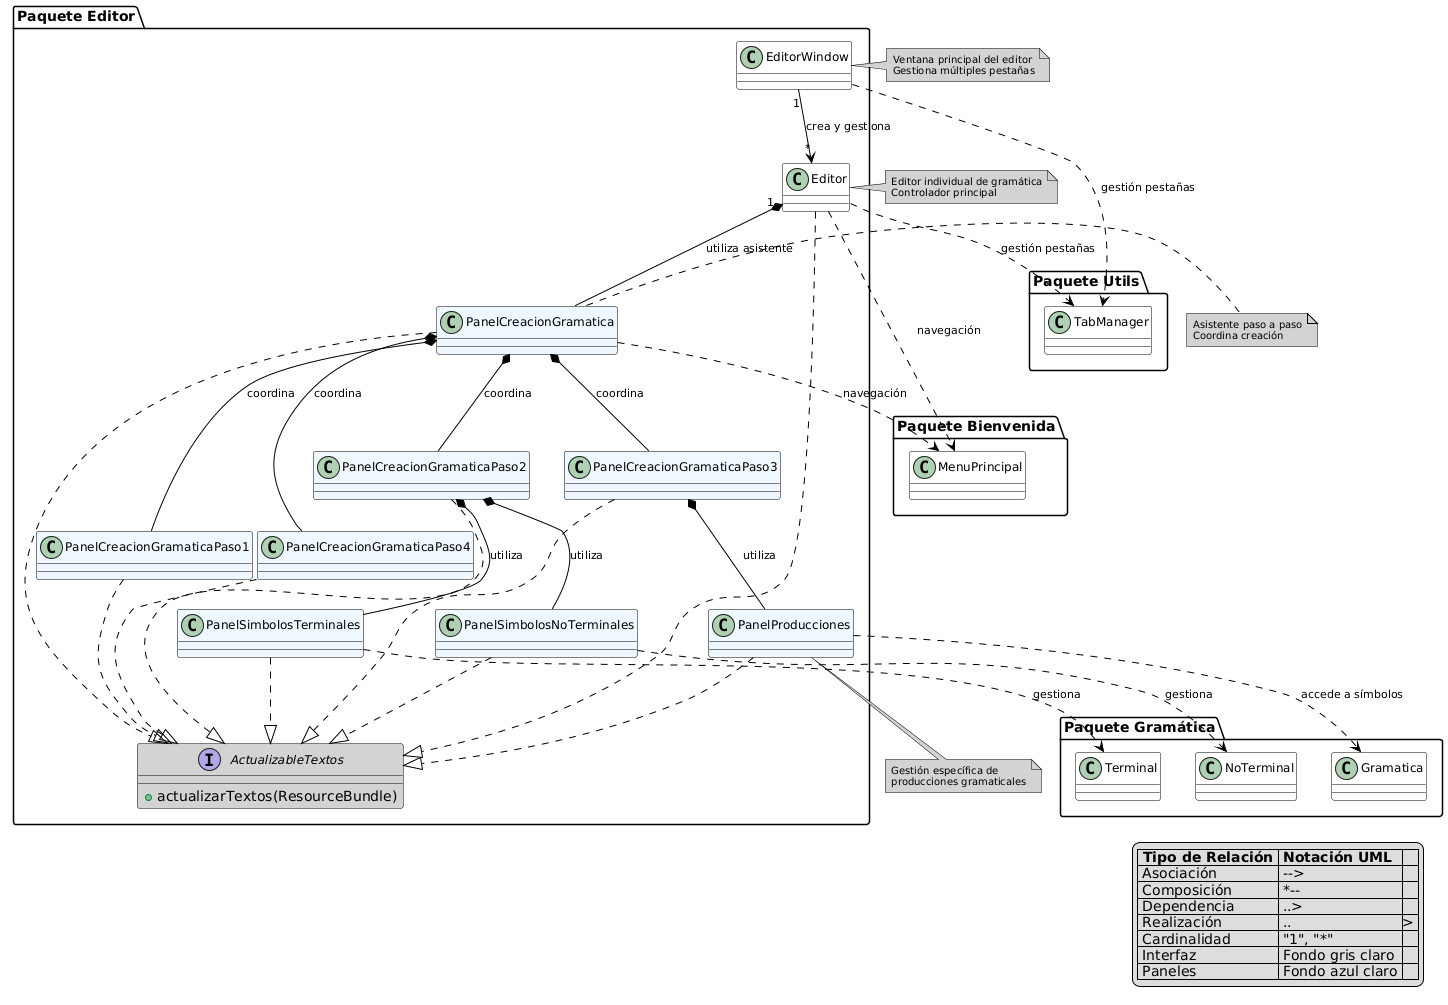
\includegraphics[angle=90,width=0.95\textwidth]{figuras/Cap9/diagrama_editor.png}
    \caption{Diagrama de clases del paquete editor - SimAS 3.0}
    \label{fig:diagrama_editor}
\end{figure}

\subsection{Paquete simulador}

El paquete \textbf{simulador} contiene las clases responsables de la simulación del análisis sintáctico descendente en SimAS 3.0. Este paquete implementa el núcleo funcional de la aplicación, permitiendo a los usuarios simular paso a paso el proceso de análisis sintáctico de cadenas de entrada utilizando gramáticas libres de contexto.

Las clases de este paquete permiten:
\begin{itemize}
    \item Simulación completa del análisis sintáctico descendente
    \item Visualización paso a paso del proceso de análisis
    \item Gestión de funciones de error y recuperación
    \item Creación y edición de cadenas de entrada
    \item Interfaz interactiva para la simulación
    \item Generación de informes y árboles de derivación
\end{itemize}

\subsubsection{Clases del paquete simulador}

Este paquete contiene 13 clases principales que implementan el sistema completo de simulación de análisis sintáctico, organizadas por funcionalidad: interfaz de pasos, clases principales de simulación, pasos de la simulación descendente y componentes auxiliares.

\subsubsection{Interfaz PanelNuevaSimDescPaso}

La interfaz \textbf{PanelNuevaSimDescPaso} define el contrato que deben implementar todos los pasos de la simulación descendente.

\begin{longtable}[H]{|>{\columncolor[rgb]{0.63,0.79,0.95}}m{6cm} | m{8.5cm} |}
\caption{Interfaz PanelNuevaSimDescPaso - Interfaz de pasos de simulación}
\endfirsthead
\multicolumn{2}{c}{{\tablename\ \thetable{} -- continúa de la página anterior}} \\
\endhead
\hline \multicolumn{2}{|r|}{{Continúa en la página siguiente}} \\ \hline
\endfoot
\hline
\endlastfoot
\hline
\textbf{Nombre} & \textbf{PanelNuevaSimDescPaso} \\ \hline
\textbf{Descripción} & Interfaz que define el contrato para todos los pasos de la simulación descendente, asegurando consistencia en la implementación. \\ \hline
\textbf{Métodos} &
\begin{enumerate}
    \item \textbf{getRoot()}: retorna el nodo raíz del paso de simulación.
\end{enumerate}
\label{tabla_panel_nueva_sim_desc_paso}
\end{longtable}

\subsubsection{Clase PanelNuevaSimDescPaso1}

La clase \textbf{PanelNuevaSimDescPaso1} implementa el primer paso de la simulación descendente, mostrando la gramática original y permitiendo la navegación entre pasos.

\begin{longtable}[H]{|>{\columncolor[rgb]{0.63,0.79,0.95}}m{6cm} | m{8.5cm} |}
\caption{Clase PanelNuevaSimDescPaso1 - Paso 1 de simulación}
\endfirsthead
\multicolumn{2}{c}{{\tablename\ \thetable{} -- continúa de la página anterior}} \\
\endhead
\hline \multicolumn{2}{|r|}{{Continúa en la página siguiente}} \\ \hline
\endfoot
\hline
\endlastfoot
\hline
\textbf{Nombre} & \textbf{PanelNuevaSimDescPaso1} \\ \hline
\textbf{Descripción} & Implementa el primer paso de la simulación descendente, mostrando la gramática original y permitiendo navegación entre los diferentes pasos del proceso. \\ \hline
\textbf{Atributos} &
\begin{enumerate}
    \item \textbf{panelPadre}: PanelSimuladorDesc que contiene este paso.
    \item \textbf{gramatica}: Gramatica que se está simulando.
    \item \textbf{bundle}: ResourceBundle para internacionalización.
    \item \textbf{root}: Parent que representa la interfaz gráfica del paso.
\end{enumerate} \\ \hline
\textbf{Métodos} &
\begin{enumerate}
    \item \textbf{PanelNuevaSimDescPaso1( PanelSimuladorDesc)}: constructor que inicializa el paso con su panel padre.
    \item \textbf{getRoot()}: retorna el nodo raíz de la interfaz gráfica.
    \item \textbf{actualizarTextos(ResourceBundle)}: actualiza los textos según el idioma seleccionado.
    \item \textbf{cargarFXML()}: carga el archivo FXML correspondiente al paso.
    \item \textbf{inicializarBotones()}: configura los botones de navegación.
\end{enumerate}
\label{tabla_panel_nueva_sim_desc_paso1}
\end{longtable}

\subsubsection{Clase PanelNuevaSimDescPaso2}

La clase \textbf{PanelNuevaSimDescPaso2} implementa el segundo paso de la simulación descendente, mostrando los símbolos terminales y no terminales.

\begin{longtable}[H]{|>{\columncolor[rgb]{0.63,0.79,0.95}}m{6cm} | m{8.5cm} |}
\caption{Clase PanelNuevaSimDescPaso2 - Paso 2 de simulación}
\endfirsthead
\multicolumn{2}{c}{{\tablename\ \thetable{} -- continúa de la página anterior}} \\
\endhead
\hline \multicolumn{2}{|r|}{{Continúa en la página siguiente}} \\ \hline
\endfoot
\hline
\endlastfoot
\hline
\textbf{Nombre} & \textbf{PanelNuevaSimDescPaso2} \\ \hline
\textbf{Descripción} & Implementa el segundo paso de la simulación descendente, mostrando los símbolos terminales y no terminales de la gramática. \\ \hline
\textbf{Atributos} &
\begin{enumerate}
    \item \textbf{panelPadre}: PanelSimuladorDesc que contiene este paso.
    \item \textbf{gramatica}: Gramatica que se está simulando.
    \item \textbf{bundle}: ResourceBundle para internacionalización.
    \item \textbf{root}: Parent que representa la interfaz gráfica del paso.
\end{enumerate} \\ \hline
\textbf{Métodos} &
\begin{enumerate}
    \item \textbf{PanelNuevaSimDescPaso2( PanelSimuladorDesc)}: constructor que inicializa el paso con su panel padre.
    \item \textbf{getRoot()}: retorna el nodo raíz de la interfaz gráfica.
    \item \textbf{actualizarTextos(ResourceBundle)}: actualiza los textos según el idioma seleccionado.
\end{enumerate}
\label{tabla_panel_nueva_sim_desc_paso2}
\end{longtable}

\subsubsection{Clase PanelNuevaSimDescPaso3}

La clase \textbf{PanelNuevaSimDescPaso3} implementa el tercer paso de la simulación descendente, mostrando los conjuntos First y Follow.

\begin{longtable}[H]{|>{\columncolor[rgb]{0.63,0.79,0.95}}m{6cm} | m{8.5cm} |}
\caption{Clase PanelNuevaSimDescPaso3 - Paso 3 de simulación}
\endfirsthead
\multicolumn{2}{c}{{\tablename\ \thetable{} -- continúa de la página anterior}} \\
\endhead
\hline \multicolumn{2}{|r|}{{Continúa en la página siguiente}} \\ \hline
\endfoot
\hline
\endlastfoot
\hline
\textbf{Nombre} & \textbf{PanelNuevaSimDescPaso3} \\ \hline
\textbf{Descripción} & Implementa el tercer paso de la simulación descendente, mostrando los conjuntos First y Follow de los símbolos no terminales. \\ \hline
\textbf{Atributos} &
\begin{enumerate}
    \item \textbf{panelPadre}: PanelSimuladorDesc que contiene este paso.
    \item \textbf{gramatica}: Gramatica que se está simulando.
    \item \textbf{bundle}: ResourceBundle para internacionalización.
    \item \textbf{root}: Parent que representa la interfaz gráfica del paso.
\end{enumerate} \\ \hline
\textbf{Métodos} &
\begin{enumerate}
    \item \textbf{PanelNuevaSimDescPaso3( PanelSimuladorDesc)}: constructor que inicializa el paso con su panel padre.
    \item \textbf{getRoot()}: retorna el nodo raíz de la interfaz gráfica.
    \item \textbf{actualizarTextos(ResourceBundle)}: actualiza los textos según el idioma seleccionado.
\end{enumerate}
\label{tabla_panel_nueva_sim_desc_paso3}
\end{longtable}

\subsubsection{Clase PanelNuevaSimDescPaso4}

La clase \textbf{PanelNuevaSimDescPaso4} implementa el cuarto paso de la simulación descendente, mostrando la tabla predictiva.

\begin{longtable}[H]{|>{\columncolor[rgb]{0.63,0.79,0.95}}m{6cm} | m{8.5cm} |}
\caption{Clase PanelNuevaSimDescPaso4 - Paso 4 de simulación}
\endfirsthead
\multicolumn{2}{c}{{\tablename\ \thetable{} -- continúa de la página anterior}} \\
\endhead
\hline \multicolumn{2}{|r|}{{Continúa en la página siguiente}} \\ \hline
\endfoot
\hline
\endlastfoot
\hline
\textbf{Nombre} & \textbf{PanelNuevaSimDescPaso4} \\ \hline
\textbf{Descripción} & Implementa el cuarto paso de la simulación descendente, mostrando la tabla predictiva completa con sus celdas y funciones de error. \\ \hline
\textbf{Atributos} &
\begin{enumerate}
    \item \textbf{panelPadre}: PanelSimuladorDesc que contiene este paso.
    \item \textbf{gramatica}: Gramatica que se está simulando.
    \item \textbf{bundle}: ResourceBundle para internacionalización.
    \item \textbf{root}: Parent que representa la interfaz gráfica del paso.
\end{enumerate} \\ \hline
\textbf{Métodos} &
\begin{enumerate}
    \item \textbf{PanelNuevaSimDescPaso4( PanelSimuladorDesc)}: constructor que inicializa el paso con su panel padre.
    \item \textbf{getRoot()}: retorna el nodo raíz de la interfaz gráfica.
    \item \textbf{funcionError()}: gestiona las funciones de error de la gramática.
    \item \textbf{reordenarIndicesFuncionesError()}: reordena los índices de las funciones de error.
    \item \textbf{actualizarTextos(ResourceBundle)}: actualiza los textos según el idioma seleccionado.
\end{enumerate}
\label{tabla_panel_nueva_sim_desc_paso4}
\end{longtable}

\subsubsection{Clase PanelNuevaSimDescPaso5}

La clase \textbf{PanelNuevaSimDescPaso5} implementa el quinto paso de la simulación descendente, permitiendo la edición de funciones de error.

\begin{longtable}[H]{|>{\columncolor[rgb]{0.63,0.79,0.95}}m{6cm} | m{8.5cm} |}
\caption{Clase PanelNuevaSimDescPaso5 - Paso 5 de simulación}
\endfirsthead
\multicolumn{2}{c}{{\tablename\ \thetable{} -- continúa de la página anterior}} \\
\endhead
\hline \multicolumn{2}{|r|}{{Continúa en la página siguiente}} \\ \hline
\endfoot
\hline
\endlastfoot
\hline
\textbf{Nombre} & \textbf{PanelNuevaSimDescPaso5} \\ \hline
\textbf{Descripción} & Implementa el quinto paso de la simulación descendente, permitiendo la edición y configuración de funciones de error para recuperación de errores. \\ \hline
\textbf{Atributos} &
\begin{enumerate}
    \item \textbf{panelPadre}: PanelSimuladorDesc que contiene este paso.
    \item \textbf{gramatica}: Gramatica que se está simulando.
    \item \textbf{bundle}: ResourceBundle para internacionalización.
    \item \textbf{root}: Parent que representa la interfaz gráfica del paso.
\end{enumerate} \\ \hline
\textbf{Métodos} &
\begin{enumerate}
    \item \textbf{PanelNuevaSimDescPaso5( PanelSimuladorDesc)}: constructor que inicializa el paso con su panel padre.
    \item \textbf{getRoot()}: retorna el nodo raíz de la interfaz gráfica.
    \item \textbf{funcionErrorToString(FuncionError)}: convierte una función de error a string para mostrar.
    \item \textbf{refrescarVista()}: refresca la vista de la tabla predictiva.
    \item \textbf{guardarDatosTabla()}: guarda los datos de la tabla predictiva.
    \item \textbf{getFuncionErrorSeleccionada()}: obtiene la función de error seleccionada.
    \item \textbf{getBundle()}: obtiene el ResourceBundle para internacionalización.
    \item \textbf{actualizarTextos(ResourceBundle)}: actualiza los textos según el idioma seleccionado.
\end{enumerate}
\label{tabla_panel_nueva_sim_desc_paso5}
\end{longtable}

\subsubsection{Clase PanelNuevaSimDescPaso6}

La clase \textbf{PanelNuevaSimDescPaso6} implementa el sexto y último paso de la simulación descendente, que corresponde al \textbf{Simulador} principal donde se ejecuta la simulación completa del análisis sintáctico.

\begin{longtable}[H]{|>{\columncolor[rgb]{0.63,0.79,0.95}}m{6cm} | m{8.5cm} |}
\caption{Clase PanelNuevaSimDescPaso6 - Paso 6 (Simulador) de simulación}
\endfirsthead
\multicolumn{2}{c}{{\tablename\ \thetable{} -- continúa de la página anterior}} \\
\endhead
\hline \multicolumn{2}{|r|}{{Continúa en la página siguiente}} \\ \hline
\endfoot
\hline
\endlastfoot
\hline
\textbf{Nombre} & \textbf{ PanelNuevaSimDescPaso6} \\ \hline
\textbf{Descripción} & Implementa el sexto y último paso de la simulación descendente (el Simulador principal), permitiendo ejecutar la simulación completa del análisis sintáctico. \\ \hline
\textbf{Atributos} &
\begin{enumerate}
    \item \textbf{panelPadre}: PanelSimuladorDesc que contiene este paso.
    \item \textbf{gramatica}: Gramatica que se está simulando.
    \item \textbf{bundle}: ResourceBundle para internacionalización.
    \item \textbf{root}: Parent que representa la interfaz gráfica del paso.
\end{enumerate} \\ \hline
\textbf{Métodos} &
\begin{enumerate}
    \item \textbf{PanelNuevaSimDescPaso6( Gramatica, PanelSimuladorDesc)}: constructor principal con gramática y panel padre.
    \item \textbf{PanelNuevaSimDescPaso6( Gramatica)}: constructor alternativo con solo gramática.
    \item \textbf{getRoot()}: retorna el nodo raíz de la interfaz gráfica.
    \item \textbf{actualizarVisualizacion()}: actualiza la visualización de la simulación.
    \item \textbf{actualizarTextos(ResourceBundle)}: actualiza los textos según el idioma seleccionado.
\end{enumerate}
\label{tabla_panel_nueva_sim_desc_paso6}
\end{longtable}

\subsubsection{Clase PanelSimuladorDesc}

La clase \textbf{PanelSimuladorDesc} es el controlador principal para la simulación descendente, coordinando todos los pasos del proceso de análisis sintáctico.

\begin{longtable}[H]{|>{\columncolor[rgb]{0.63,0.79,0.95}}m{6cm} | m{8.5cm} |}
\caption{Clase PanelSimuladorDesc - Controlador principal de simulación}
\endfirsthead
\multicolumn{2}{c}{{\tablename\ \thetable{} -- continúa de la página anterior}} \\
\endhead
\hline \multicolumn{2}{|r|}{{Continúa en la página siguiente}} \\ \hline
\endfoot
\hline
\endlastfoot
\hline
\textbf{Nombre} & \textbf{PanelSimuladorDesc} \\ \hline
\textbf{Descripción} & Controlador principal que coordina toda la simulación descendente, gestionando los diferentes pasos, la gramática y la interacción con el usuario. \\ \hline
\textbf{Atributos} &
\begin{enumerate}
    \item \textbf{tabPane}: TabPane donde se muestran los pasos de simulación.
    \item \textbf{gramatica}: Gramatica que se está simulando.
    \item \textbf{gramaticaOriginal}: copia independiente de la gramática original.
    \item \textbf{pasoActual}: número del paso actual en la simulación.
    \item \textbf{pasos}: ArrayList con todos los pasos de la simulación.
    \item \textbf{bundle}: ResourceBundle para internacionalización.
    \item \textbf{tablaPredictivaExtendidaGlobal}: TablaPredictivaPaso5 con funciones de error.
    \item \textbf{simuladorId}: identificador único del simulador.
    \item \textbf{simuladoresActivos}: Map estático con todos los simuladores activos.
\end{enumerate} \\ \hline
\textbf{Métodos} &
\begin{enumerate}
    \item \textbf{PanelSimuladorDesc(Gramatica, TabPane, ResourceBundle)}: constructor principal.
    \item \textbf{PanelSimuladorDesc(Gramatica, TabPane, ResourceBundle, String)}: constructor con ID personalizado.
    \item \textbf{PanelSimuladorDesc(Gramatica, TabPane, MenuPrincipal, String, ResourceBundle)}: constructor completo.
    \item \textbf{getTablaPredictivaExtendidaGlobal()}: obtiene la tabla predictiva extendida global.
    \item \textbf{setTablaPredictivaExtendidaGlobal( TablaPredictivaPaso5)}: establece la tabla predictiva extendida global.
    \item \textbf{getGramaticaOriginal()}: obtiene la gramática original.
    \item \textbf{mostrarGramaticaOriginal()}: muestra la gramática original.
    \item \textbf{cancelarSimulacion()}: cancela la simulación actual.
    \item \textbf{cambiarPaso(int)}: cambia al paso especificado.
    \item \textbf{cerrarPestañaFuncionesError()}: cierra la pestaña de funciones de error.
    \item \textbf{getBundle()}: obtiene el ResourceBundle.
    \item \textbf{setBundle(ResourceBundle)}: establece el ResourceBundle.
    \item \textbf{getRoot()}: obtiene el nodo raíz.
    \item \textbf{getPasoActual()}: obtiene el paso actual.
    \item \textbf{configurarRelacionesPadreHijo()}: configura las relaciones padre-hijo.
    \item \textbf{getSimuladorId()}: obtiene el ID único del simulador.
\end{enumerate} \\ \hline
\textbf{Métodos Estáticos} &
\begin{enumerate}
    \item \textbf{actualizarTodosLosSimuladores( ResourceBundle)}: actualiza todos los simuladores activos.
    \item \textbf{desregistrarSimulador(String)}: desregistra un simulador del registro global.
    \item \textbf{obtenerSimulador(String)}: obtiene un simulador por su ID.
\end{enumerate}
\label{tabla_panel_simulador_desc}
\end{longtable}

\subsubsection{Clase PanelSimulacion}

La clase \textbf{PanelSimulacion} implementa un panel completo para la simulación interactiva del análisis sintáctico.

\begin{longtable}[H]{|>{\columncolor[rgb]{0.63,0.79,0.95}}m{6cm} | m{8.5cm} |}
\caption{Clase PanelSimulacion - Panel de simulación interactiva}
\endfirsthead
\multicolumn{2}{c}{{\tablename\ \thetable{} -- continúa de la página anterior}} \\
\endhead
\hline \multicolumn{2}{|r|}{{Continúa en la página siguiente}} \\ \hline
\endfoot
\hline
\endlastfoot
\hline
\textbf{Nombre} & \textbf{PanelSimulacion} \\ \hline
\textbf{Descripción} & Panel que proporciona una interfaz completa para la simulación interactiva del análisis sintáctico, permitiendo controlar paso a paso el proceso de análisis. \\ \hline
\textbf{Atributos} &
\begin{enumerate}
    \item \textbf{gramatica}: Gramatica que se está simulando.
    \item \textbf{tablaPredictiva}: TablaPredictivaPaso5 con funciones de error.
    \item \textbf{funcionesError}: List de FuncionError disponibles.
    \item \textbf{entrada}: String que representa la cadena de entrada.
    \item \textbf{pila}: Stack que simula la pila del analizador.
    \item \textbf{entradaActual}: List que contiene los símbolos de entrada.
    \item \textbf{posicionEntrada}: posición actual en la cadena de entrada.
    \item \textbf{simulacionEnCurso}: boolean que indica si la simulación está activa.
    \item \textbf{bundle}: ResourceBundle para internacionalización.
\end{enumerate} \\ \hline
\textbf{Métodos} &
\begin{enumerate}
    \item \textbf{PanelSimulacion(Gramatica, ResourceBundle)}: constructor que inicializa el panel de simulación.
    \item \textbf{getRoot()}: obtiene el componente raíz VBox de la interfaz.
\end{enumerate}
\label{tabla_panel_simulacion}
\end{longtable}

\subsubsection{Clase SimulacionFinal}

La clase \textbf{SimulacionFinal} implementa la simulación completa del análisis sintáctico con capacidades avanzadas de visualización y control.

\begin{longtable}[H]{|>{\columncolor[rgb]{0.63,0.79,0.95}}m{6cm} | m{8.5cm} |}
\caption{Clase SimulacionFinal - Simulación completa avanzada}
\endfirsthead
\multicolumn{2}{c}{{\tablename\ \thetable{} -- continúa de la página anterior}} \\
\endhead
\hline \multicolumn{2}{|r|}{{Continúa en la página siguiente}} \\ \hline
\endfoot
\hline
\endlastfoot
\hline
\textbf{Nombre} & \textbf{SimulacionFinal} \\ \hline
\textbf{Descripción} & Implementa la simulación completa del análisis sintáctico con capacidades avanzadas como historial, navegación, generación de informes y visualización de árboles de derivación. \\ \hline
\textbf{Atributos} &
\begin{enumerate}
    \item \textbf{gramatica}: Gramatica que se está simulando.
    \item \textbf{tablaPredictiva}: TablaPredictivaPaso5 con funciones de error.
    \item \textbf{funcionesError}: List de FuncionError para recuperación.
    \item \textbf{pila}: Stack que simula la pila del analizador.
    \item \textbf{entradaActual}: ArrayList con la cadena de entrada.
    \item \textbf{historialPasos}: ObservableList con el historial de pasos.
    \item \textbf{pasoActual}: posición actual en la simulación.
    \item \textbf{bundle}: ResourceBundle para internacionalización.
\end{enumerate} \\ \hline
\textbf{Métodos} &
\begin{enumerate}
    \item \textbf{SimulacionFinal(Gramatica, TablaPredictivaPaso5, TabPane, ResourceBundle)}: constructor principal.
    \item \textbf{setSimulacionId(String)}: establece el ID único de la simulación.
    \item \textbf{actualizarGrupoYTitulo()}: actualiza el grupo y título de la simulación.
    \item \textbf{actualizarTitulosPestañas(int, boolean, int, boolean)}: actualiza títulos de pestañas con parámetros.
    \item \textbf{actualizarTitulosPestañas()}: actualiza títulos de pestañas sin parámetros.
    \item \textbf{perteneceASimulador(String)}: verifica si pertenece a un simulador específico.
    \item \textbf{esHijaDeLaSimulacion(Tab)}: verifica si una pestaña es hija de la simulación.
    \item \textbf{getSimuladorPadreId()}: obtiene el ID del simulador padre.
    \item \textbf{setGrupoId(String)}: establece el ID del grupo.
    \item \textbf{setNumeroGrupo(int)}: establece el número del grupo.
    \item \textbf{getGrupoId()}: obtiene el ID del grupo.
    \item \textbf{getNumeroGrupo()}: obtiene el número del grupo.
    \item \textbf{actualizarTextos(ResourceBundle)}: actualiza textos según el idioma.
\end{enumerate}
\label{tabla_simulacion_final}
\end{longtable}

\subsubsection{Clase PanelGramaticaOriginal}

La clase \textbf{PanelGramaticaOriginal} muestra la gramática original en una pestaña separada con soporte para internacionalización.

\begin{longtable}[H]{|>{\columncolor[rgb]{0.63,0.79,0.95}}m{6cm} | m{8.5cm} |}
\caption{Clase PanelGramaticaOriginal - Panel de gramática original}
\endfirsthead
\multicolumn{2}{c}{{\tablename\ \thetable{} -- continúa de la página anterior}} \\
\endhead
\hline \multicolumn{2}{|r|}{{Continúa en la página siguiente}} \\ \hline
\endfoot
\hline
\endlastfoot
\hline
\textbf{Nombre} & \textbf{PanelGramaticaOriginal} \\ \hline
\textbf{Descripción} & Panel que muestra la gramática original en una pestaña separada, permitiendo visualizar todas las producciones de forma clara y organizada. \\ \hline
\textbf{Atributos} &
\begin{enumerate}
    \item \textbf{gramaticaOriginal}: Gramatica original que se muestra.
    \item \textbf{bundle}: ResourceBundle para internacionalización.
\end{enumerate} \\ \hline
\textbf{Métodos} &
\begin{enumerate}
    \item \textbf{PanelGramaticaOriginal(Gramatica, ResourceBundle)}: constructor que inicializa el panel.
    \item \textbf{getRoot()}: retorna el nodo raíz del panel.
    \item \textbf{actualizarTextos(ResourceBundle)}: actualiza los textos según el idioma seleccionado.
\end{enumerate}
\label{tabla_panel_gramatica_original}
\end{longtable}

\subsubsection{Clase NuevaFuncionError}

La clase \textbf{NuevaFuncionError} permite crear y configurar nuevas funciones de error para la recuperación en el análisis sintáctico.

\begin{longtable}[H]{|>{\columncolor[rgb]{0.63,0.79,0.95}}m{6cm} | m{8.5cm} |}
\caption{Clase NuevaFuncionError - Creación de funciones de error}
\endfirsthead
\multicolumn{2}{c}{{\tablename\ \thetable{} -- continúa de la página anterior}} \\
\endhead
\hline \multicolumn{2}{|r|}{{Continúa en la página siguiente}} \\ \hline
\endfoot
\hline
\endlastfoot
\hline
\textbf{Nombre} & \textbf{NuevaFuncionError} \\ \hline
\textbf{Descripción} & Permite crear y configurar nuevas funciones de error para la recuperación automática durante el análisis sintáctico descendente. \\ \hline
\textbf{Atributos} &
\begin{enumerate}
    \item \textbf{gramatica}: Gramatica donde se aplicarán las funciones de error.
    \item \textbf{paso4}: PanelNuevaSimDescPaso4 que contiene este componente.
    \item \textbf{bundle}: ResourceBundle para internacionalización.
    \item \textbf{root}: Parent que representa la interfaz gráfica.
\end{enumerate} \\ \hline
\textbf{Métodos} &
\begin{enumerate}
    \item \textbf{NuevaFuncionError(Gramatica, PanelNuevaSimDescPaso4, ResourceBundle)}: constructor principal.
    \item \textbf{getRoot()}: retorna el nodo raíz de la interfaz.
    \item \textbf{actualizarTextos(ResourceBundle)}: actualiza los textos según el idioma seleccionado.
\end{enumerate}
\label{tabla_nueva_funcion_error}
\end{longtable}

\subsubsection{Clase EditorCadenaEntradaController}

La clase \textbf{EditorCadenaEntradaController} proporciona una interfaz para editar y gestionar las cadenas de entrada que se utilizarán en la simulación.

\begin{longtable}[H]{|>{\columncolor[rgb]{0.63,0.79,0.95}}m{6cm} | m{8.5cm} |}
\caption{Clase EditorCadenaEntradaController - Editor de cadenas de entrada}
\endfirsthead
\multicolumn{2}{c}{{\tablename\ \thetable{} -- continúa de la página anterior}} \\
\endhead
\hline \multicolumn{2}{|r|}{{Continúa en la página siguiente}} \\ \hline
\endfoot
\hline
\endlastfoot
\hline
\textbf{Nombre} & \textbf{EditorCadenaEntradaController} \\ \hline
\textbf{Descripción} & Controlador FXML que gestiona la edición de cadenas de entrada mediante una interfaz gráfica con lista de terminales disponibles y campo de texto para composición de la cadena. \\ \hline
\textbf{Atributos} &
\begin{enumerate}
    \item \textbf{stage}: Stage que contiene la ventana del editor.
    \item \textbf{resultado}: String que contiene el resultado final de la edición.
\end{enumerate} \\ \hline
\textbf{Métodos} &
\begin{enumerate}
    \item \textbf{setStage(Stage)}: establece la referencia al Stage de la ventana.
    \item \textbf{setTerminales(List<Terminal>)}: establece la lista de terminales disponibles.
    \item \textbf{setCadenaInicial(String)}: establece la cadena inicial en el campo de texto.
    \item \textbf{getResultado()}: obtiene el resultado final de la edición.
\end{enumerate}
\label{tabla_editor_cadena_entrada_controller}
\end{longtable}

\subsubsection{Dependencias internas del paquete simulador}

Las dependencias internas del paquete simulador se ilustran en la Figura \ref{fig:diagrama_simulador}, donde se puede apreciar la estructura organizada del sistema de simulación paso a paso y sus interacciones con otros paquetes.

\begin{itemize}
    \item \textbf{PanelSimuladorDesc $\rightarrow$ PanelNuevaSimDescPaso1-6}: PanelSimuladorDesc contiene y coordina todos los pasos de simulación, siendo PanelNuevaSimDescPaso6 el Simulador principal.
    \item \textbf{PanelNuevaSimDescPaso1-6 $\rightarrow$ PanelNuevaSimDescPaso}: todos los pasos implementan la interfaz PanelNuevaSimDescPaso.
    \item \textbf{PanelSimuladorDesc $\leftrightarrow$ Gramatica}: utiliza la gramática para la simulación.
    \item \textbf{PanelSimuladorDesc $\leftrightarrow$ TablaPredictivaPaso5}: utiliza la tabla predictiva extendida.
    \item \textbf{SimulacionFinal $\rightarrow$ Gramatica}: utiliza la gramática para simulación completa.
    \item \textbf{PanelSimulacion $\rightarrow$ TablaPredictivaPaso5}: utiliza la tabla predictiva para simulación interactiva.
    \item \textbf{NuevaFuncionError $\rightarrow$ PanelNuevaSimDescPaso4}: se integra en el paso 4 de la simulación.
    \item \textbf{PanelGramaticaOriginal $\rightarrow$ Gramatica}: muestra la gramática original.
    \item \textbf{EditorCadenaEntradaController $\rightarrow$ Gramatica}: valida cadenas contra la gramática.
    \item \textbf{Todas las clases $\rightarrow$ ResourceBundle}: utilizan internacionalización.
\end{itemize}

\begin{figure}[p]
    \centering
    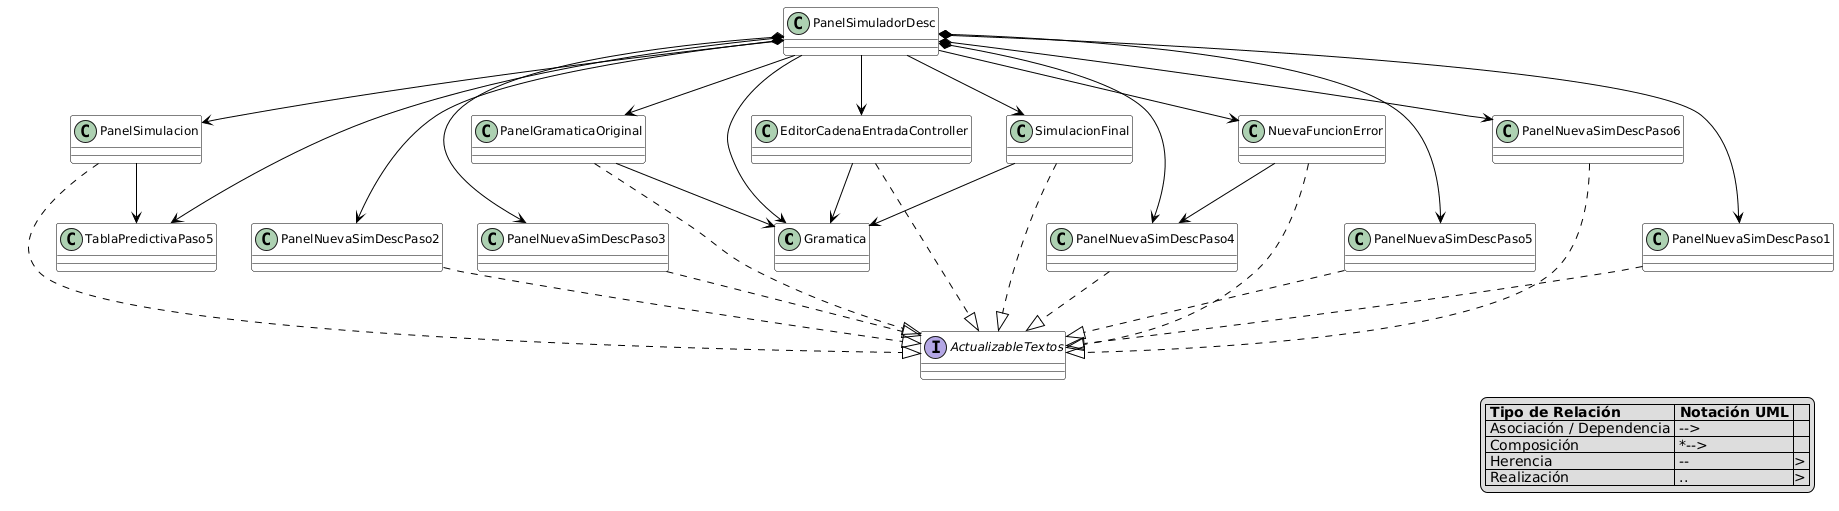
\includegraphics[angle=90,width=\textwidth,height=\textheight]{figuras/Cap9/diagrama_simulador2.png}
    \caption{Diagrama de dependencias del paquete simulador - SimAS 3.0}
    \label{fig:diagrama_simulador}
\end{figure}

\subsubsection{Patrones de diseño en el paquete simulador}

\begin{itemize}
    \item \textbf{MVC (Model-View-Controller)}: el paquete sigue el patrón MVC donde las clases del paquete gramática son el Modelo, las clases del simulador son los Controladores, y los componentes FXML son las Vistas \cite{burbeck1992applications}.
    \item \textbf{Strategy}: los diferentes pasos de simulación (PanelNuevaSimDescPaso1-6) implementan estrategias diferentes para cada fase del análisis \cite{gamma1995design}.
    \item \textbf{Observer}: las clases implementan ActualizableTextos para observar cambios en el idioma y actualizar automáticamente la interfaz \cite{gamma1995design}.
    \item \textbf{Factory Method}: los constructores de PanelSimuladorDesc crean diferentes configuraciones de simuladores según los parámetros \cite{gamma1995design}.
    \item \textbf{Registry}: PanelSimuladorDesc mantiene un registro estático de todos los simuladores activos para gestión centralizada.
\end{itemize}

\section{Paquetes de soporte}

\subsection{Paquete centroayuda}

El paquete \textbf{centroayuda} contiene recursos y componentes relacionados con el sistema de ayuda y tutoriales de la aplicación SimAS 3.0. Este paquete incluye:

\begin{itemize}
    \item \textbf{Contenido HTML}: archivos de ayuda interactiva y tutoriales accesibles desde la aplicación.
    \item \textbf{Recursos multimedia}: imágenes, diagramas y elementos visuales que complementan la documentación.
    \item \textbf{Archivos PDF}: manuales técnicos y guías de usuario en formato PDF para consulta offline.
    \item \textbf{Documentación integrada}: sistema de ayuda contextual que se activa desde diferentes puntos de la interfaz.
\end{itemize}

Este paquete proporciona soporte integral al usuario, desde tutoriales interactivos hasta documentación técnica detallada, facilitando el aprendizaje y uso efectivo de la aplicación.

\subsection{Paquete vistas}

El paquete \textbf{vistas} contiene todos los archivos de interfaz de usuario definidos en formato FXML (JavaFX XML), que constituyen la capa de presentación de la aplicación SimAS 3.0. Este paquete incluye:

\begin{itemize}
    \item \textbf{Archivos FXML principales}: definiciones de las interfaces principales como Bienvenida, MenuPrincipal y Editor.
    \item \textbf{Componentes reutilizables}: paneles y controles personalizados utilizados en múltiples secciones.
    \item \textbf{Interfaces de simulación}: archivos FXML para cada paso del proceso de simulación descendente.
    \item \textbf{Hojas de estilo}: archivos CSS que definen el aspecto visual y temas de la aplicación.
\end{itemize}

Este paquete implementa completamente la separación entre lógica de negocio y presentación visual, siguiendo el patrón MVC. Una descripción más detallada de la estructura FXML, organización de componentes y diseño de interfaces se presenta en el Capítulo 10 de este manual.

\subsection{Paquete resources}

El paquete \textbf{resources} centraliza todos los recursos estáticos y elementos multimedia utilizados por la aplicación SimAS 3.0. Este paquete incluye:

\begin{itemize}
    \item \textbf{Imágenes de interfaz}: iconos, botones y elementos gráficos utilizados en la interfaz de usuario.
    \item \textbf{Recursos de internacionalización}: archivos de propiedades (.properties) para soporte multiidioma (español, inglés, francés, japonés, portugués).
    \item \textbf{Elementos visuales}: imágenes decorativas, logos y componentes gráficos de la aplicación.
    \item \textbf{Archivos de configuración}: recursos adicionales necesarios para el funcionamiento correcto de la aplicación.
\end{itemize}

Este paquete garantiza que todos los recursos necesarios estén organizados de manera eficiente y sean fácilmente accesibles desde cualquier parte de la aplicación, facilitando el mantenimiento y actualización de elementos visuales e internacionalización.

\section{Dependencias entre Paquetes}

Esta sección presenta un análisis detallado de las dependencias entre los diferentes paquetes del sistema SimAS 3.0, mostrando cómo se interconectan las clases para formar una arquitectura coherente y modular.

\subsection{Dependencias Detalladas por Paquete}

\subsubsection{Dependencias del paquete bienvenida}

\begin{itemize}
    \item \textbf{bienvenida.Bienvenida $\rightarrow$ bienvenida.MenuPrincipal}: la clase Bienvenida transita automáticamente al MenuPrincipal después de mostrar la pantalla de bienvenida.
    \item \textbf{bienvenida.MenuPrincipal $\rightarrow$ editor.EditorWindow}: MenuPrincipal crea instancias de EditorWindow para iniciar editores.
    \item \textbf{bienvenida.MenuPrincipal $\rightarrow$ simulador.PanelSimuladorDesc}: MenuPrincipal crea instancias del simulador descendente.
    \item \textbf{bienvenida.MenuPrincipal $\rightarrow$ utils.TabManager}: MenuPrincipal utiliza TabManager para gestión avanzada de pestañas.
    \item \textbf{bienvenida.MenuPrincipal $\rightarrow$ utils.LanguageItem}: MenuPrincipal utiliza LanguageItem para el selector de idiomas.
    \item \textbf{bienvenida.MenuPrincipal $\rightarrow$ java.util.ResourceBundle}: MenuPrincipal gestiona la internacionalización mediante ResourceBundle.
    \item \textbf{bienvenida.MenuPrincipal $\rightarrow$ utils.SecondaryWindow}: MenuPrincipal puede crear ventanas secundarias para gestión de pestañas.
    \item \textbf{bienvenida.MenuPrincipal $\rightarrow$ centroayuda}: MenuPrincipal accede a recursos de ayuda cuando el usuario solicita asistencia.
\end{itemize}

\subsubsection{Dependencias del paquete editor}

\begin{itemize}
    \item \textbf{editor.* $\rightarrow$ gramatica.Gramatica}: todas las clases del editor utilizan la clase Gramatica como modelo de datos central.
    \item \textbf{editor.* $\rightarrow$ utils.TabManager}: las clases del editor utilizan TabManager para gestión de pestañas y grupos.
    \item \textbf{editor.* $\rightarrow$ utils.ActualizableTextos}: las clases del editor implementan esta interfaz para internacionalización.
    \item \textbf{editor.PanelCreacionGramatica $\rightarrow$ editor.PanelCreacionGramaticaPaso*}: PanelCreacionGramatica coordina todos los pasos del asistente.
    \item \textbf{editor.* $\rightarrow$ bienvenida.MenuPrincipal}: las clases del editor referencian al MenuPrincipal para navegación.
    \item \textbf{editor.PanelProducciones $\rightarrow$ gramatica.Produccion}: PanelProducciones gestiona objetos Produccion.
    \item \textbf{editor.PanelSimbolos* $\rightarrow$ gramatica.Terminal/NoTerminal}: los paneles de símbolos gestionan terminales y no terminales.
    \item \textbf{editor.* $\rightarrow$ utils.ResourceBundle}: las clases del editor utilizan recursos de internacionalización.
\end{itemize}

\subsubsection{Dependencias del paquete gramática}

\begin{itemize}
    \item \textbf{gramatica.* $\rightarrow$ gramatica.Simbolo}: todas las clases gramaticales heredan o utilizan la clase base Simbolo.
    \item \textbf{gramatica.Gramatica $\rightarrow$ gramatica.Terminal/NoTerminal/Produccion}: Gramatica contiene colecciones de estos elementos.
    \item \textbf{gramatica.Gramatica $\rightarrow$ gramatica.TablaPredictiva}: Gramatica utiliza TablaPredictiva para análisis sintáctico.
    \item \textbf{gramatica.TablaPredictiva $\rightarrow$ gramatica.FilaTablaPredictiva}: TablaPredictiva contiene filas de tabla predictiva.
    \item \textbf{gramatica.TablaPredictiva $\rightarrow$ gramatica.FuncionError}: TablaPredictiva gestiona funciones de error.
    \item \textbf{gramatica.TablaPredictivaPaso5 $\rightarrow$ gramatica.TablaPredictiva}: herencia y extensión de funcionalidad.
    \item \textbf{gramatica.* $\rightarrow$ java.util.ObservableList}: las clases gramaticales utilizan ObservableList para notificación automática.
\end{itemize}

\subsubsection{Dependencias del paquete simulador}

\begin{itemize}
    \item \textbf{simulador.* $\rightarrow$ gramatica.Gramatica}: todas las clases del simulador utilizan Gramatica como modelo.
    \item \textbf{simulador.* $\rightarrow$ gramatica.TablaPredictivaPaso5}: los simuladores utilizan la tabla predictiva extendida.
    \item \textbf{simulador.PanelSimuladorDesc $\rightarrow$ simulador.PanelNuevaSimDescPaso*}: PanelSimuladorDesc coordina todos los pasos.
    \item \textbf{simulador.PanelNuevaSimDescPaso* $\rightarrow$ simulador.PanelNuevaSimDescPaso}: implementan la interfaz común.
    \item \textbf{simulador.* $\rightarrow$ utils.ActualizableTextos}: las clases del simulador implementan internacionalización.
    \item \textbf{simulador.PanelNuevaSimDescPaso4 $\rightarrow$ simulador.NuevaFuncionError}: Paso 4 utiliza NuevaFuncionError para gestión de errores.
    \item \textbf{simulador.* $\rightarrow$ utils.TabManager}: los simuladores utilizan gestión de pestañas.
    \item \textbf{simulador.* $\rightarrow$ utils.ResourceBundle}: los simuladores utilizan recursos de internacionalización.
\end{itemize}

\subsubsection{Dependencias del paquete utils}

\begin{itemize}
    \item \textbf{utils.TabManager $\rightarrow$ utils.TabPaneMonitor}: TabManager utiliza el monitor para supervisión.
    \item \textbf{utils.SecondaryWindow $\rightarrow$ utils.TabManager}: SecondaryWindow utiliza gestión de pestañas.
    \item \textbf{utils.* $\rightarrow$ utils.ActualizableTextos}: las clases utils implementan o utilizan esta interfaz.
    \item \textbf{utils.TabPaneMonitor $\rightarrow$ javafx.scene.control.TabPane}: el monitor supervisa TabPanes.
    \item \textbf{utils.* $\rightarrow$ java.util.ResourceBundle}: las clases utils utilizan internacionalización.
    \item \textbf{utils.LanguageItem $\rightarrow$ java.util.ResourceBundle}: LanguageItem utiliza recursos de idioma.
\end{itemize}

\subsubsection{Dependencias transversales del sistema}

\begin{itemize}
    \item \textbf{Todos los paquetes $\rightarrow$ utils.ActualizableTextos}: interfaz implementada por clases de todos los paquetes para internacionalización.
    \item \textbf{Todos los paquetes $\rightarrow$ java.util.ResourceBundle}: todos los paquetes utilizan recursos de internacionalización.
    \item \textbf{Todos los paquetes $\rightarrow$ utils.TabManager}: gestión centralizada de pestañas utilizada por múltiples paquetes.
    \item \textbf{Paquet vista $\rightarrow$ Todos los paquetes}: los archivos FXML referencian controladores de todos los paquetes.
    \item \textbf{Paquet resources $\rightarrow$ Todos los paquetes}: recursos utilizados por clases de todos los paquetes.
\end{itemize}

\subsection{Análisis de acoplamiento}

\subsubsection{Acoplamiento bajo (recomendable)}
\begin{itemize}
    \item \textbf{Interfaces}: el uso de interfaces como \texttt{ActualizableTextos} y \texttt{PanelNuevaSimDescPaso} reduce el acoplamiento.
    \item \textbf{Inyección de dependencias}: las clases reciben sus dependencias a través de constructores, facilitando testing.
    \item \textbf{Patrones de diseño}: MVC, Strategy, Observer y Factory Method promueven bajo acoplamiento.
\end{itemize}

\subsubsection{Acoplamiento alto (áreas de atención)}
\begin{itemize}
    \item \textbf{Dependencia circular}: algunos paquetes tienen dependencias bidireccionales que podrían refactorizarse.
    \item \textbf{Dependencias transversales}: ResourceBundle y TabManager son utilizados por muchos paquetes.
    \item \textbf{Dependencias específicas}: algunas clases tienen dependencias muy específicas que limitan la reutilización.
\end{itemize}

\subsection{Principios SOLID aplicados}

En esta sección se analiza la aplicación de los principios SOLID (Single Responsibility, Open-Closed, Liskov Substitution, Interface Segregation, Dependency Inversion) en la arquitectura de SimAS 3.0, con referencias específicas a clases concretas y fundamentación teórica.

\subsubsection{Principio de Responsabilidad Única (SRP)}

El Principio de Responsabilidad Única establece que una clase debe tener una sola razón para cambiar, es decir, debe tener una única responsabilidad \cite{martin2003agile, martin2018clean}.

\begin{itemize}
    \item \textbf{Clase gramatica.Gramatica}: responsable únicamente de gestionar la lógica de datos de una gramática (terminales, no terminales, producciones). No maneja presentación ni persistencia.
    \begin{itemize}
        \item \textit{Ejemplo}: métodos como \texttt{validarGramatica()}, \texttt{generarConjPrim()}, \texttt{generarConjSig()} se centran exclusivamente en la lógica gramatical.
    \end{itemize}

    \item \textbf{Clase utils.TabManager}: responsable únicamente de la gestión centralizada de pestañas y grupos. No conoce detalles específicos de editores o simuladores.
    \begin{itemize}
        \item \textit{Ejemplo}: métodos como \texttt{getOrCreateTab()}, \texttt{asignarElementoANuevoGrupo()} manejan exclusivamente lógica de pestañas.
    \end{itemize}

    \item \textbf{Clase editor.PanelCreacionGramatica}: responsable únicamente de coordinar el asistente de creación paso a paso. No implementa la lógica de cada paso.
    \begin{itemize}
        \item \textit{Ejemplo}: método \texttt{cambiarPaso(int)} coordina navegación, mientras que cada PanelCreacionGramaticaPaso* implementa su propio paso.
    \end{itemize}

    \item \textbf{Clase simulador.PanelSimuladorDesc}: responsable únicamente de orquestar la simulación descendente. No implementa la lógica de cada paso individual.
    \begin{itemize}
        \item \textit{Ejemplo}: gestiona el estado global de la simulación (\texttt{pasoActual}, \texttt{pasos}) sin conocer detalles de análisis sintáctico.
    \end{itemize}
\end{itemize}

\subsubsection{Principio de Abierto/Cerrado (OCP)}

El Principio de Abierto/Cerrado establece que las entidades de software deben estar abiertas para extensión pero cerradas para modificación \cite{meyer1988object, martin2003agile}.

\begin{itemize}
    \item \textbf{Interfaz simulador.PanelNuevaSimDescPaso}: permite agregar nuevos pasos de simulación sin modificar el código existente del simulador principal.
    \begin{itemize}
        \item \textit{Ejemplo}: para agregar un nuevo paso 7, solo se crea una clase \texttt{PanelNuevaSimDescPaso7} que implemente la interfaz, sin modificar \texttt{PanelSimuladorDesc}.
    \end{itemize}

    \item \textbf{Interfaz utils.ActualizableTextos}: permite agregar internacionalización a cualquier clase sin modificar su implementación interna.
    \begin{itemize}
        \item \textit{Ejemplo}: cualquier clase puede implementar \texttt{actualizarTextos(ResourceBundle)} para soporte multiidioma sin cambiar su lógica principal.
    \end{itemize}

    \item \textbf{Clase gramatica.TablaPredictiva}: puede extenderse con nuevas estrategias de análisis sin modificar la implementación base.
    \begin{itemize}
        \item \textit{Ejemplo}: \texttt{TablaPredictivaPaso5} extiende \texttt{TablaPredictiva} agregando funcionalidad específica para el paso 5 del simulador.
    \end{itemize}

    \item \textbf{Clase utils.TabManager}: puede manejar nuevos tipos de pestañas sin modificar su lógica central.
    \begin{itemize}
        \item \textit{Ejemplo}: método \texttt{getOrCreateTab(Class<?> tabType, ...)} acepta cualquier tipo de controlador, permitiendo extensión sin modificación.
    \end{itemize}
\end{itemize}

\subsubsection{Principio de Sustitución de Liskov (LSP)}

El Principio de Sustitución de Liskov establece que los objetos de una clase derivada deben poder sustituirse por objetos de la clase base sin afectar la corrección del programa \cite{liсков1994program, martin2003agile}.

\begin{itemize}
    \item \textbf{Jerarquía gramatica.Simbolo}: las clases \texttt{Terminal} y \texttt{NoTerminal} pueden sustituirse por \texttt{Simbolo} en cualquier contexto.
    \begin{itemize}
        \item \textit{Ejemplo}: en \texttt{Gramatica.getTerminales()} y \texttt{Gramatica.getNoTerminales()}, ambos retornan \texttt{ObservableList<? extends Simbolo>}, permitiendo tratamiento uniforme.
    \end{itemize}

    \item \textbf{Implementaciones de PanelNuevaSimDescPaso}: cualquier implementación de la interfaz puede sustituirse por otra sin afectar \texttt{PanelSimuladorDesc}.
    \begin{itemize}
        \item \textit{Ejemplo}: \texttt{PanelNuevaSimDescPaso1} puede reemplazarse por cualquier otra implementación sin modificar el código del simulador principal.
    \end{itemize}

    \item \textbf{Clases de pasos de creación}: los diferentes \texttt{PanelCreacionGramaticaPaso*} pueden sustituirse entre sí manteniendo compatibilidad.
    \begin{itemize}
        \item \textit{Ejemplo}: cualquier paso del asistente puede reemplazarse por otro que implemente la misma interfaz sin afectar \texttt{PanelCreacionGramatica}.
    \end{itemize}

    \item \textbf{Implementaciones de ActualizableTextos}: cualquier clase que implemente la interfaz puede utilizarse donde se espere internacionalización.
    \begin{itemize}
        \item \textit{Ejemplo}: tanto \texttt{Editor} como \texttt{PanelSimuladorDesc} implementan la interfaz y pueden tratarse uniformemente para cambios de idioma.
    \end{itemize}
\end{itemize}

\subsubsection{Principio de Segregación de Interfaces (ISP)}

El Principio de Segregación de Interfaces establece que los clientes no deben verse forzados a depender de interfaces que no utilizan \cite{martin2003agile, martin2018clean}.

\begin{itemize}
    \item \textbf{Interfaz utils.ActualizableTextos}: interfaz específica y minimalista solo para internacionalización.
    \begin{itemize}
        \item \textit{Ejemplo}: solo declara \texttt{actualizarTextos(ResourceBundle)}, evitando forzar a las clases a implementar métodos innecesarios de internacionalización compleja.
    \end{itemize}

    \item \textbf{Interfaz simulador.PanelNuevaSimDescPaso}: interfaz minimalista solo para la estructura de pasos de simulación.
    \begin{itemize}
        \item \textit{Ejemplo}: solo declara \texttt{getRoot()}, evitando obligar a los pasos a implementar métodos de navegación o estado que maneja el coordinador.
    \end{itemize}

    \item \textbf{Clase utils.TabManager}: proporciona métodos específicos separados en lugar de una interfaz monolítica.
    \begin{itemize}
        \item \textit{Ejemplo}: métodos como \texttt{isSimuladorContent()}, \texttt{isEditorContent()} permiten a los clientes usar solo la funcionalidad necesaria.
    \end{itemize}

    \item \textbf{Ausencia de interfaces infladas}: las clases evitan depender de interfaces con métodos no utilizados.
    \begin{itemize}
        \item \textit{Ejemplo}: \texttt{Editor} no implementa interfaces con métodos de simulación que no necesita, manteniendo separación clara de responsabilidades.
    \end{itemize}
\end{itemize}

\subsubsection{Principio de Inversión de Dependencias (DIP)}

El Principio de Inversión de Dependencias establece que los módulos de alto nivel no deben depender de módulos de bajo nivel, sino que ambos deben depender de abstracciones \cite{martin2003agile, martin2018clean}.

\begin{itemize}
    \item \textbf{Dependencias de interfaces en lugar de clases concretas}: las clases dependen de interfaces, no de implementaciones concretas.
    \begin{itemize}
        \item \textit{Ejemplo}: \texttt{PanelSimuladorDesc} depende de \texttt{PanelNuevaSimDescPaso} (interfaz), no de implementaciones concretas como \texttt{PanelNuevaSimDescPaso1}.
    \end{itemize}

    \item \textbf{Inyección de dependencias a través de constructores}: las clases reciben sus dependencias externas en lugar de crearlas internamente.
    \begin{itemize}
        \item \textit{Ejemplo}: \texttt{Editor(TabPane, MenuPrincipal, ResourceBundle)} recibe todas sus dependencias, facilitando testing y reutilización.
        \item \textit{Ejemplo}: \texttt{PanelSimuladorDesc(Gramatica, TabPane, ResourceBundle)} permite inyectar diferentes implementaciones.
    \end{itemize}

    \item \textbf{Dependencia de abstracciones}: las clases de alto nivel dependen de interfaces, no de implementaciones concretas.
    \begin{itemize}
        \item \textit{Ejemplo}: \texttt{MenuPrincipal} depende de \texttt{utils.ActualizableTextos} (interfaz) para internacionalización, no de implementaciones específicas.
    \end{itemize}

    \item \textbf{Fábricas y constructores parametrizados}: permiten crear diferentes configuraciones sin violar DIP.
    \begin{itemize}
        \item \textit{Ejemplo}: los múltiples constructores de \texttt{PanelSimuladorDesc} permiten diferentes configuraciones manteniendo la dependencia de interfaces.
    \end{itemize}
\end{itemize}

\subsection{Evaluación de Calidad Arquitectural}

\subsubsection{Métricas de Acoplamiento y Cohesión}

Basado en el análisis de dependencias, la arquitectura presenta:

\begin{itemize}
    \item \textbf{Cohesión Alta}: cada paquete tiene responsabilidades claramente definidas
    \begin{itemize}
        \item Paquete \texttt{gramatica}: cohesión máxima en lógica gramatical
        \item Paquete \texttt{utils}: cohesión máxima en utilidades transversales
        \item Paquete \texttt{editor}: cohesión máxima en interfaces de edición
    \end{itemize}

    \item \textbf{Acoplamiento Controlado}: uso estratégico de interfaces reduce acoplamiento
    \begin{itemize}
        \item Acoplamiento a través de interfaces (\texttt{PanelNuevaSimDescPaso}, \texttt{ActualizableTextos})
        \item Inyección de dependencias reduce acoplamiento temporal
        \item Patrones Observer y Strategy mantienen bajo acoplamiento
    \end{itemize}

    \item \textbf{Complejidad Ciclomática Aceptable}: separación clara de responsabilidades
    \begin{itemize}
        \item Clases con responsabilidades únicas tienen baja complejidad
        \item Coordinadores (como \texttt{PanelSimuladorDesc}) manejan complejidad de integración
    \end{itemize}
\end{itemize}

\subsubsection{Puntos Fuertes de la Arquitectura}

\begin{itemize}
    \item \textbf{Mantenibilidad}: principios SOLID facilitan modificaciones localizadas
    \item \textbf{Testabilidad}: inyección de dependencias permite mock objects
    \item \textbf{Reutilización}: interfaces permiten uso polimórfico
    \item \textbf{Escalabilidad}: OCP permite agregar funcionalidad sin modificar código existente
    \item \textbf{Comprensibilidad}: separación clara de responsabilidades facilita comprensión
\end{itemize}

\subsubsection{Áreas de Mejora Identificadas}

\begin{itemize}
    \item \textbf{Dependencias transversales}: \texttt{TabManager} y \texttt{ResourceBundle} podrían refactorizarse para reducir acoplamiento
    \item \textbf{Complejidad de constructores}: algunos constructores tienen muchos parámetros, podrían beneficiarse de Builder Pattern
    \item \textbf{Dependencias circulares}: algunas relaciones bidireccionales podrían eliminarse con eventos o mediadores
\end{itemize}

\section{Conclusiones}

Este capítulo ha presentado un análisis exhaustivo de la arquitectura de clases de SimAS 3.0, demostrando una implementación robusta de principios de diseño orientado a objetos y patrones de diseño reconocidos. La estructura modular y bien organizada facilita el mantenimiento, extensión y comprensión del sistema.

Los paquetes principales (bienvenida, editor, gramática, simulador, utils) han sido analizados en detalle, mostrando cómo cada componente cumple con responsabilidades específicas mientras mantiene una cohesión adecuada y un acoplamiento flexible. Los paquetes de soporte (centroayuda, vistas, resources) complementan esta arquitectura proporcionando recursos esenciales para la experiencia del usuario.

La implementación del patrón MVC, junto con otros patrones como Strategy, Observer, Factory Method y Registry, demuestra un diseño profesional que facilita la evolución del software y su adaptación a nuevos requisitos. La documentación detallada de atributos y métodos asegura que cualquier desarrollador pueda comprender y extender el sistema de manera efectiva.

En el siguiente capítulo se profundizará en la capa de presentación (paquete vistas), analizando en detalle los archivos FXML y el diseño de interfaces de usuario que complementan esta arquitectura de clases.
